\documentclass[conference]{IEEEtran}
\IEEEoverridecommandlockouts
\usepackage{cite}
\usepackage{amsmath,amssymb,amsfonts}
\usepackage{textcomp}
\usepackage{xcolor}
\usepackage{balance}
\usepackage{booktabs}
\usepackage{float}
\usepackage{graphicx,url}
\usepackage{soulutf8,color}
\usepackage{stfloats}
\usepackage{verbatim}
\usepackage[utf8]{inputenc}
\usepackage[inline]{enumitem}
\usepackage{multirow}
\usepackage{array}
\usepackage{tikz}
\usepackage{hyperref}

\renewcommand{\abstractname}{Resumo}
\renewcommand{\refname}{REFERÊNCIAS}

\begin{document}

\title{Seleção Zero-Touch de Algoritmos de Virtual Network Embedding usando Árvores de Decisão Multi-Objetivo}

\author{\IEEEauthorblockN{Luis Antonio Momm Duarte}
\IEEEauthorblockA{\textit{Programa de Pós-Graduação em Computação Aplicada} \\
\textit{Universidade do Estado de Santa Catarina}\\
Joinville, Brasil \\
luis.duarte@edu.udesc.br}
}

\maketitle

\begin{abstract}
O problema de \textit{Virtual Network Embedding} (VNE) é fundamental em infraestruturas de nuvem nas quais múltiplos provedores compartilham recursos físicos. O mapeamento de requisições de redes virtuais sobre a infraestrutura física, satisfazendo restrições de capacidade e otimizando objetivos como taxa de aceitação e consumo de recursos, é NP-difícil, motivando o desenvolvimento de diversos algoritmos que variam desde métodos exatos baseados em Programação Inteira Mista (MIP) até heurísticas e meta-heurísticas. Contudo, nenhum algoritmo apresenta desempenho superior em todos os cenários. Este trabalho propõe uma abordagem baseada em árvores de decisão multi-objetivo para selecionar automaticamente o algoritmo VNE mais apropriado para cada requisição, considerando o estado da rede física e características da requisição. O método emprega três modelos especializados, cada um otimizado para um objetivo específico (taxa de aceitação, razão receita-custo e receita média), permitindo adaptação às prioridades operacionais em tempo de execução. A validação experimental em três topologias de \textit{datacenter} com 8.000 requisições apresenta \textit{top-3 accuracy} entre 79,1\% e 85,9\% na predição do melhor algoritmo, com melhoria de +32,9 pontos percentuais na taxa de aceitação em relação ao \textit{baseline} de algoritmo fixo. A abordagem oferece interpretabilidade através de caminhos de decisão explícitos, latência de inferência inferior a 1\,ms viabilizando operação \textit{online}, e capacidade de operação autônoma alinhada aos requisitos de administração \textit{zero-touch}.
\end{abstract}

\begin{IEEEkeywords}
Virtual Network Embedding, Árvores de Decisão, Otimização Multi-Objetivo, Administração Zero-Touch, Machine Learning Interpretável
\end{IEEEkeywords}

%===================================================================

\section{Introdução}
\label{sec:Intro}

O problema de \textit{Virtual Network Embedding} (VNE) emergiu como habilitador essencial para redes modernas, incluindo \textit{datacenters} em nuvem, computação em borda (\textit{edge computing}) e redes 5G, devido à sua flexibilidade e escalabilidade. O VNE tornou-se crítico em infraestruturas nas quais múltiplos provedores de serviço compartilham recursos de rede física. O problema aborda o desafio de mapear requisições de redes virtuais (VNRs) sobre a infraestrutura física, satisfazendo restrições de capacidade e otimizando objetivos como taxa de aceitação, tempo de processamento e consumo de energia.

Nas últimas duas décadas, numerosos algoritmos de VNE foram propostos, variando desde métodos exatos baseados em Programação Inteira Mista (MIP) até heurísticas e meta-heurísticas.
Um desafio fundamental permanece: \textbf{nenhum algoritmo único apresenta desempenho consistentemente superior em todos os cenários}~\cite{fischer2013vne-survey}.
Diferentes características de VNRs (tamanho, topologia, demandas) e estados da rede física (utilização, fragmentação de recursos) demandam algoritmos distintos.

Abordagens tradicionais de implantação de VNE tipicamente selecionam um único algoritmo para todas as requisições, independentemente de suas características ou do estado atual da rede. Esta estratégia falha em explorar os pontos fortes de diferentes algoritmos para cenários específicos.

Adicionalmente, a administração \textit{zero-touch} de redes virtualizadas tornou-se requisito crítico em infraestruturas modernas.
O conceito de \textit{Zero-Touch Network and Service Management} (ZSM), formalizado pelo padrão ETSI desde 2017~\cite{etsi-zsm}, refere-se à capacidade de sistemas operarem de forma autônoma através de mecanismos de controle programável, virtualização e retroalimentação de malha fechada, com mínima intervenção humana.
Pesquisas da indústria indicam que redes autônomas podem reduzir custos operacionais significativamente.
Contudo, a lacuna entre pesquisa e implantação permanece: enquanto sistemas de \textit{Reinforcement Learning} (RL) profundo e otimização atingem desempenho elevado, carecem de interpretabilidade e sofrem com latência de decisão inadequada para sistemas de tempo real~\cite{white2024zerotough}.
Portanto, sistemas que realizam seleção automática de algoritmos VNE sem intervenção do operador são fundamentais para alcançar operação verdadeiramente autônoma.

Neste contexto, o presente trabalho propõe uma abordagem baseada em \textbf{árvores de decisão multi-objetivo} para selecionar automaticamente o algoritmo VNE mais apropriado para cada requisição, considerando o estado da rede e características da requisição.
Diferentemente de um modelo único, o método emprega três modelos especializados, cada um otimizado para um objetivo específico (taxa de aceitação, razão receita-custo, receita média), permitindo adaptação às prioridades operacionais em tempo de execução, com latência de inferência inferior a 1\,ms viabilizando operação \textit{online}.

O manuscrito está organizado da seguinte forma: a Seção~\ref{sec:RefTeo} apresenta o referencial teórico; a Seção~\ref{sec:RelatedWork} discute trabalhos relacionados; a Seção~\ref{sec:Proposal} descreve a metodologia proposta; a Seção~\ref{sec:Results} apresenta resultados experimentais; e a Seção~\ref{sec:Conclusion} conclui o artigo.

\section{\textit{Background} e Motivação}
\label{sec:RefTeo}

Esta seção apresenta os conceitos fundamentais para compreensão do problema de VNE e das técnicas de \textit{machine learning} empregadas.
A Subseção~\ref{subsec:vne} descreve o problema de VNE e suas classes de algoritmos.
A Subseção~\ref{subsec:trees} introduz árvores de decisão como mecanismo de seleção.
A Subseção~\ref{subsec:multiobj} discute otimização multi-objetivo.

\subsection{\textit{Virtual Network Embedding}}
\label{subsec:vne}

\textit{Virtual Network Embedding} (VNE) é o processo de mapear requisições de redes virtuais sobre uma infraestrutura de rede física compartilhada.
Uma requisição de rede virtual $G_v = (N_v, L_v)$ consiste em um conjunto de nós virtuais $N_v$ e enlaces virtuais $L_v$, sendo que cada nó e enlace possui demandas de recursos específicas (CPU, memória, largura de banda).
A rede física $G_p = (N_p, L_p)$ fornece o substrato computacional e de rede.

O problema de VNE pode ser decomposto em dois subproblemas: (i) mapeamento de nós virtuais para nós físicos; e (ii) mapeamento de enlaces virtuais para caminhos na rede física. O objetivo é maximizar métricas como taxa de aceitação de VNRs, minimizar tempo de processamento e otimizar consumo de recursos físicos.

O problema de VNE é NP-difícil~\cite{fischer2013vne-survey}, motivando o desenvolvimento de diversas classes de algoritmos:

\begin{itemize}
    \item \textbf{Algoritmos Exatos}: Métodos como Programação Inteira Mista (MIP) garantem soluções ótimas, porém possuem complexidade exponencial.
    \item \textbf{Heurísticas}: Algoritmos gulosos que tomam decisões locais baseadas em \textit{rankings} de nós, oferecendo tempo de execução reduzido com qualidade de solução variável.
    \item \textbf{Meta-heurísticas}: Técnicas como algoritmos genéticos (GA), otimização por enxame de partículas (PSO) e busca em árvore de Monte Carlo (MCTS) empregam busca estocástica que balanceia exploração e qualidade.
\end{itemize}

Dado que diferentes algoritmos VNE apresentam desempenho variável conforme o contexto, torna-se necessário um mecanismo para selecionar automaticamente o algoritmo mais apropriado. A próxima subseção apresenta árvores de decisão como técnica de \textit{machine learning} adequada para essa seleção contextual.

\subsection{Árvores de Decisão para Classificação}
\label{subsec:trees}

Dado que diversos algoritmos VNE existem e cada um é apropriado para contextos diferentes, torna-se necessário um mecanismo para aprender qual algoritmo selecionar em cada cenário. Esta subseção descreve árvores de decisão, a técnica de \textit{machine learning} empregada para realizar essa seleção.

Árvores de decisão são modelos de aprendizado supervisionado que particionam recursivamente o espaço de \textit{features} para criar regiões homogêneas de predição.
A Figura~\ref{fig:tree-structure} ilustra a estrutura geral de uma árvore de decisão.

\begin{figure}[H]
    \centering
    
\includegraphics[width=0.9\columnwidth]{tree_structure}
    \caption{Estrutura de uma árvore de decisão: particionamento recursivo do espaço de \textit{features}.}
    \label{fig:tree-structure}
\end{figure}

Conforme ilustrado na Figura~\ref{fig:tree-structure}, a árvore inicia em um nó raiz contendo todos os dados de treinamento.
Progressivamente, em cada nível, a árvore subdivide o espaço de \textit{features} usando decisões binárias, criando ramos especializados.
Cada folha (nó terminal) representa uma predição final---neste contexto, qual algoritmo VNE é mais apropriado.

Em cada nó interno, a árvore seleciona uma \textit{feature} e um \textit{threshold}, dividindo dados em dois subconjuntos. O critério de divisão utiliza índice de Gini ou ganho de informação, maximizando o isolamento de classes. Cada caminho da raiz até uma folha representa uma regra de decisão interpretável.

A Figura~\ref{fig:tree-example-path} ilustra um exemplo de caminho de decisão, mostrando como cada decisão intermediária na árvore reduz progressivamente o espaço de soluções até alcançar uma recomendação final.

\begin{figure}[H]
    \centering
    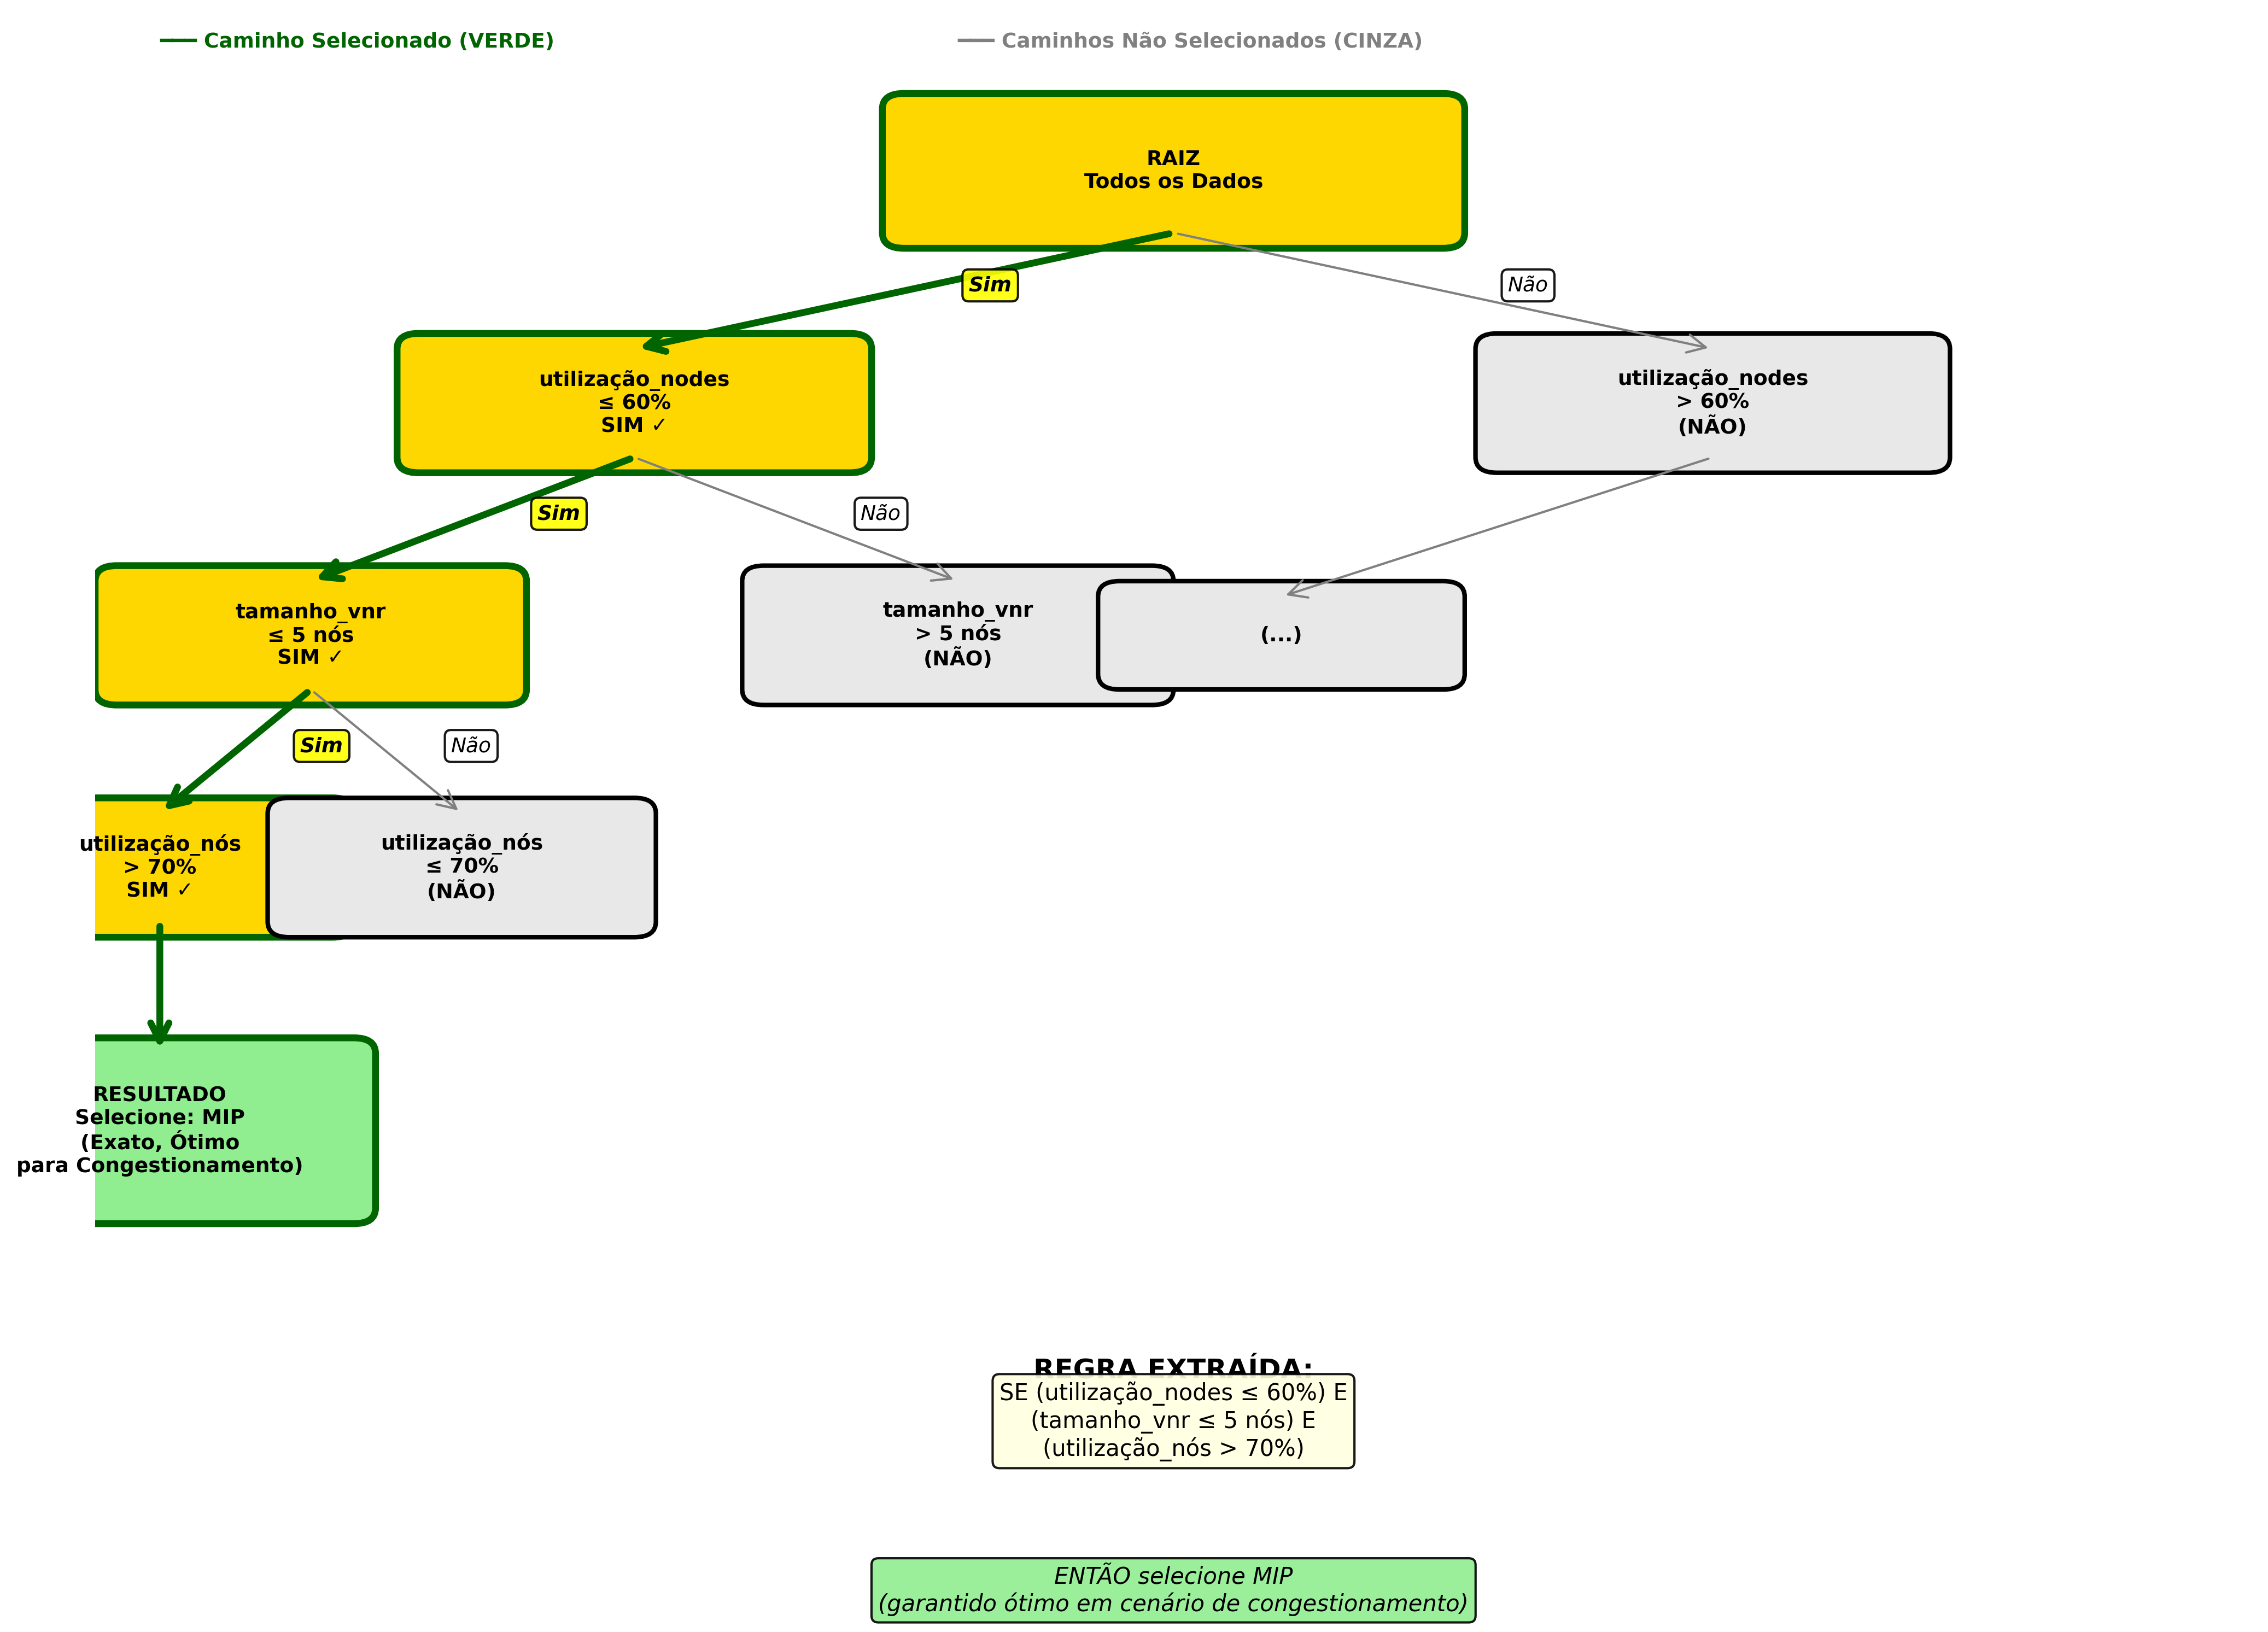
\includegraphics[width=0.95\columnwidth]{tree_example_path}
    \caption{Exemplo de caminho de decisão (raiz até folha) em árvore para seleção de algoritmo VNE.}
    \label{fig:tree-example-path}
\end{figure}

Diferentemente de redes neurais profundas ou modelos de \textit{reinforcement learning}, cada passo é compreensível e auditável por operadores humanos.
Árvores de decisão são particularmente adequadas para o problema de seleção de algoritmos VNE devido às seguintes características:

\begin{itemize}
    \item \textbf{Interpretabilidade}: Cada decisão pode ser rastreada através de um caminho lógico explícito na árvore.
    \item \textbf{Invariância a Escala}: Funcionam adequadamente com \textit{features} em escalas diferentes (CPU em unidades, utilização em porcentagem).
    \item \textbf{Baixa Latência}: Inferência possui complexidade $O(\log n)$ na profundidade, tipicamente inferior a 1\,ms.
    \item \textbf{Explicabilidade}: Operadores compreendem exatamente quais \textit{features} determinaram a decisão.
\end{itemize}

\subsection{Otimização Multi-Objetivo}
\label{subsec:multiobj}

A seleção de qual algoritmo utilizar não deve considerar apenas uma métrica de desempenho. Em ambientes reais de produção, múltiplos objetivos competem simultaneamente: taxa de aceitação de VNRs, tempo de resolução e consumo de recursos. Abordagens que otimizam um objetivo único frequentemente negligenciam outros, causando desequilíbrio no sistema. A estratégia proposta emprega múltiplas árvores especializadas, cada uma otimizada para um objetivo específico, permitindo que o sistema adapte prioridades em tempo de execução conforme requisitos operacionais.

A seção seguinte posiciona este trabalho em relação à literatura existente, analisando trabalhos relacionados em seleção de algoritmos, otimização multi-objetivo e automação de redes.

\section{Trabalhos Relacionados}
\label{sec:RelatedWork}

Esta seção posiciona o trabalho em relação à literatura existente em VNE, seleção de algoritmos e automação de redes.
A Tabela~\ref{tab:related-work} sintetiza a análise comparativa entre trabalhos relacionados e a abordagem proposta.

\subsection{Seleção de Algoritmos}
\label{subsec:alg-selection}

O problema de seleção de algoritmos foi formalizado por Rice~\cite{rice1976algorithm}, que estabeleceu o \textit{framework} conceitual: dado um espaço de problemas, um conjunto de algoritmos, um espaço de \textit{features} descritivas, e métricas de desempenho, determinar qual algoritmo é mais apropriado para cada problema. Este \textit{framework} fundamenta a abordagem proposta neste trabalho.

Xu et al.~\cite{xu2012satzilla} desenvolvem SATzilla, um seletor baseado em portfólio para problemas de satisfabilidade (SAT), mostrando que seleção dinâmica produz ganhos significativos sobre algoritmos únicos. De forma relacionada, Koslowski et al.~\cite{koslowski2025knowledge-based} aplicam técnicas de \textit{machine learning} para seleção adaptativa de políticas de escalonamento em infraestruturas de computação de alto desempenho (HPC), mostrando que consolidação de múltiplas estratégias oferece adaptabilidade superior. Este paradigma aplica-se igualmente ao domínio de VNE. A próxima subseção discute como a otimização multi-objetivo tem sido abordada em trabalhos relacionados de redes virtualizadas.

\subsection{Otimização Multi-Objetivo em Redes}
\label{subsec:multiobj-networks}

Realidades operacionais de redes modernas demandam otimização simultânea de múltiplos objetivos: taxa de aceitação, razão receita-custo, receita média e tempo de processamento. Abordagens clássicas em VNE tipicamente otimizam um objetivo singular, negligenciando \textit{trade-offs} com outros.

Song et al.~\cite{song2020multiobjective} e Belgacem et al.~\cite{belgacem2016multiobjective} exploram otimização multi-objetivo para VNE e alocação de recursos em redes virtualizadas. Contudo, estas abordagens frequentemente utilizam algoritmos evolucionários ou programação inteira dinâmica, que sofrem com complexidade computacional durante operação \textit{online}. A abordagem proposta diferencia-se ao empregar modelos independentes para cada objetivo, permitindo que operadores selecionem em tempo de execução qual prioridade otimizar.

\subsection{\textit{Machine Learning} e Aprendizado por Reforço em Redes}
\label{subsec:ml-networks}

\textit{Machine learning} tornou-se ferramenta importante para automação de redes.
Cao et al.~\cite{cao2018nfv-deeprl} aplicam \textit{Deep Reinforcement Learning} (DRL) para alocação dinâmica de recursos em NFV (\textit{Network Function Virtualization}).
Wang et al.~\cite{ijcai-2024-flagvne} propõem FlagVNE, um \textit{framework} flexível de RL para VNE com múltiplas políticas.

Embora DRL ofereça adaptatividade, enfrenta desafios críticos para produção: longo tempo de treino (milhões de episódios para convergência), falta de interpretabilidade (decisões funcionam como ``caixa preta''), convergência instável em ambientes dinâmicos, e latência de inferência elevada (inadequada para decisões em tempo real).
Trabalhos recentes em sistemas autônomos de rede reconhecem que interpretabilidade é requisito crítico para ambientes regulados~\cite{white2024zerotough}. A próxima subseção discute trabalhos relacionados especificamente em automação \textit{zero-touch}.

\subsection{Automação \textit{Zero-Touch}}
\label{subsec:zerotouchj}

O conceito de \textit{Zero-Touch Network and Service Management} (ZSM) foi formalizado pela ETSI desde 2017, referindo-se à operação de sistemas de rede com mínima intervenção humana, através de controle programável, virtualização e retroalimentação de malha fechada.

Pesquisas da indústria indicam que redução de intervenção manual pode diminuir custos operacionais em até 40\%.
Contudo, a lacuna entre pesquisa e produção permanece: sistemas de RL alcançam desempenho elevado, porém carecem de interpretabilidade adequada para operações críticas.

O RSCAT~\cite{diel2023rscat} propõe automação \textit{zero-touch} para controle de congestionamento em redes usando aprendizado por reforço \textit{actor-critic} e SDN.
RSCAT mostra que combinação de \textit{machine learning} e técnicas clássicas pode viabilizar operação autônoma, similarmente à abordagem proposta neste trabalho para seleção contextual de algoritmos VNE. A subseção seguinte sintetiza a análise comparativa entre os trabalhos relacionados e a abordagem proposta.

\subsection{Discussão}

A Tabela~\ref{tab:related-work} sintetiza uma análise comparativa entre trabalhos relacionados e a abordagem proposta segundo seis dimensões críticas para sistemas de produção:

\begin{table*}[t]
\centering
\caption{Análise Comparativa: Trabalhos Relacionados vs Abordagem Proposta (seis dimensões críticas)}
\label{tab:related-work}
\begin{tabular}{lcccccc}
\toprule
\textbf{Trabalho} & \textbf{Tipo} & \textbf{Adaptativo} & \textbf{Múltiplos} & \textbf{Interpretável} & \textbf{Latência} & \textbf{Produção} \\
                  & \textbf{ML} & \textbf{por VNR} & \textbf{Objetivos} &                       & \textbf{Inferência} & \textbf{Ready} \\
\midrule
Fischer (VNE Survey) & Comparação & Não & Não & Sim & - & Não \\
Rice (Portfólio) & Algoritmo & Sim & Não & Sim & - & Conceptual \\
SATzilla & Árvores & Sim & Não & Sim & Baixa & Sim \\
Cao et al. (DRL) & RL Profundo & Sim & Não & Não & Alta (50ms+) & Não \\
FlagVNE (DRL) & RL Profundo & Sim & Não & Não & Muito Alta (100ms+) & Não \\
\midrule
\textbf{Este Trabalho} & \textbf{Árvores Multi-Obj.} & \textbf{Sim} & \textbf{Sim (3 objetivos)} & \textbf{Sim} & \textbf{Muito Baixa <1ms} & \textbf{Sim} \\
\bottomrule
\end{tabular}
\end{table*}

Este trabalho diferencia-se ao combinar conceitos consolidados — seleção de algoritmos, árvores de decisão e otimização multi-objetivo — aplicados a VNE para criar uma solução prática e operacional. As principais contribuições distintivas incluem:
\begin{itemize}
    \item \textbf{Multi-Objetividade}: Três modelos especializados, não apenas otimização de aceitação. Operadores podem adaptar prioridades em tempo de execução conforme condições operacionais mudam.

    \item \textbf{Adaptatividade Contextual}: Seleção baseada em estado real da rede (utilização, fragmentação) e características da requisição (tamanho, conectividade), não apenas características da VNR.

    \item \textbf{Interpretabilidade Completa}: Diferentemente de abordagens de RL/DL (caixa preta), cada decisão pode ser explicada aos operadores através de caminhos explícitos na árvore de decisão.

    \item \textbf{Eficiência Computacional}: Treino em segundos (não milhões de episódios), inferência em sub-milissegundos ($<$1ms), viabilizando operação online em tempo real.

    \item \textbf{Validação Prática}: Apresenta melhoria real em taxa de aceitação (+5,73pp) em ambiente simulado realístico com 8.000 requisições de rede virtual em três topologias.
\end{itemize}

A seção seguinte detalha a metodologia proposta, descrevendo as etapas de coleta de dados, engenharia de \textit{features}, treinamento dos modelos e predição online.

\section{Metodologia}
\label{sec:Proposal}

\subsection{Visão Geral da Abordagem}

A metodologia consiste em quatro etapas principais:

\begin{enumerate}
    \item \textbf{Coleta de Dados}: Executar oito algoritmos VNE --- \textit{MIP, GA-Meta, PSO-Meta, SA-Meta, MCTS, PL-Rank, RW-Rank-BFS, D-Round} --- em três topologias distintas --- \textit{Tree, Fat-Tree (k=4) e Waxman-16} --- e coletar dados de desempenho detalhados em cada cenário para treinamento, validação e teste do modelo.
    \item \textbf{Engenharia de Features}: Extrair 27 características relevantes das VNRs, estado da rede e contexto topológico.
    \item \textbf{Treino Multi-Objetivo}: Criar três modelos especializados --- RAC (\textit{Request Acceptance Rate}, taxa de aceitação de requisições), LRC (\textit{Long-term Revenue-to-Cost Ratio}, razão receita-custo de longo prazo) e LAR (\textit{Long-term Average Revenue}, receita média de longo prazo) ---, cada um otimizando critérios específicos de desempenho.
    \item \textbf{Predição Online}: Para cada nova VNR, utilizar o contexto extraído para selecionar dinamicamente o algoritmo VNE mais adequado através do modelo que otimiza o critério desejado.
\end{enumerate}

\subsection{Geração de Dados de Simulações}

Dados foram coletados utilizando a plataforma \textbf{Virne}~\cite{wang2024virne}, um \textit{framework} abrangente de \textit{benchmarking} para problemas de alocação de recursos em NFV (\textit{Network Function Virtualization Resource Allocation}). O Virne oferece simulações altamente customizáveis para diversos cenários de rede, incluindo \textit{datacenters} em nuvem, computação em borda e redes 5G. A plataforma implementa mais de 30 algoritmos NFV-RA em uma arquitetura modular e extensível, fornecendo um ambiente de simulação \textit{event-driven} que modela a infraestrutura de rede física (PN) e requisições sequenciais de redes virtuais (VNRs). Cada chegada de VNR é tratada como um evento discreto, criando uma instância que o algoritmo NFV-RA deve resolver, avaliando a viabilidade da solução e atualizando os recursos da rede.

As simulações foram executadas com oito algoritmos VNE em três topologias distintas, comumente usadas em \textit{datacenters}:

\textbf{Topologias}:
\begin{itemize}
    \item \textbf{Tree}: Hierárquica binária com 32 hosts e 31 switches (63 nós)
    \item \textbf{Fat-Tree}: \textit{Datacenter} com k=4 (16 servidores, 20 switches, 36 nós)
    \item \textbf{Waxman-16}: Rede aleatória com 16 nós e 500 links
\end{itemize}

A Figura~\ref{fig:topologies-comparison} apresenta visualização das topologias Tree e Fat-Tree utilizadas nas simulações, mostrando suas estruturas hierárquicas distintas:

\begin{figure}[H]
    \centering
    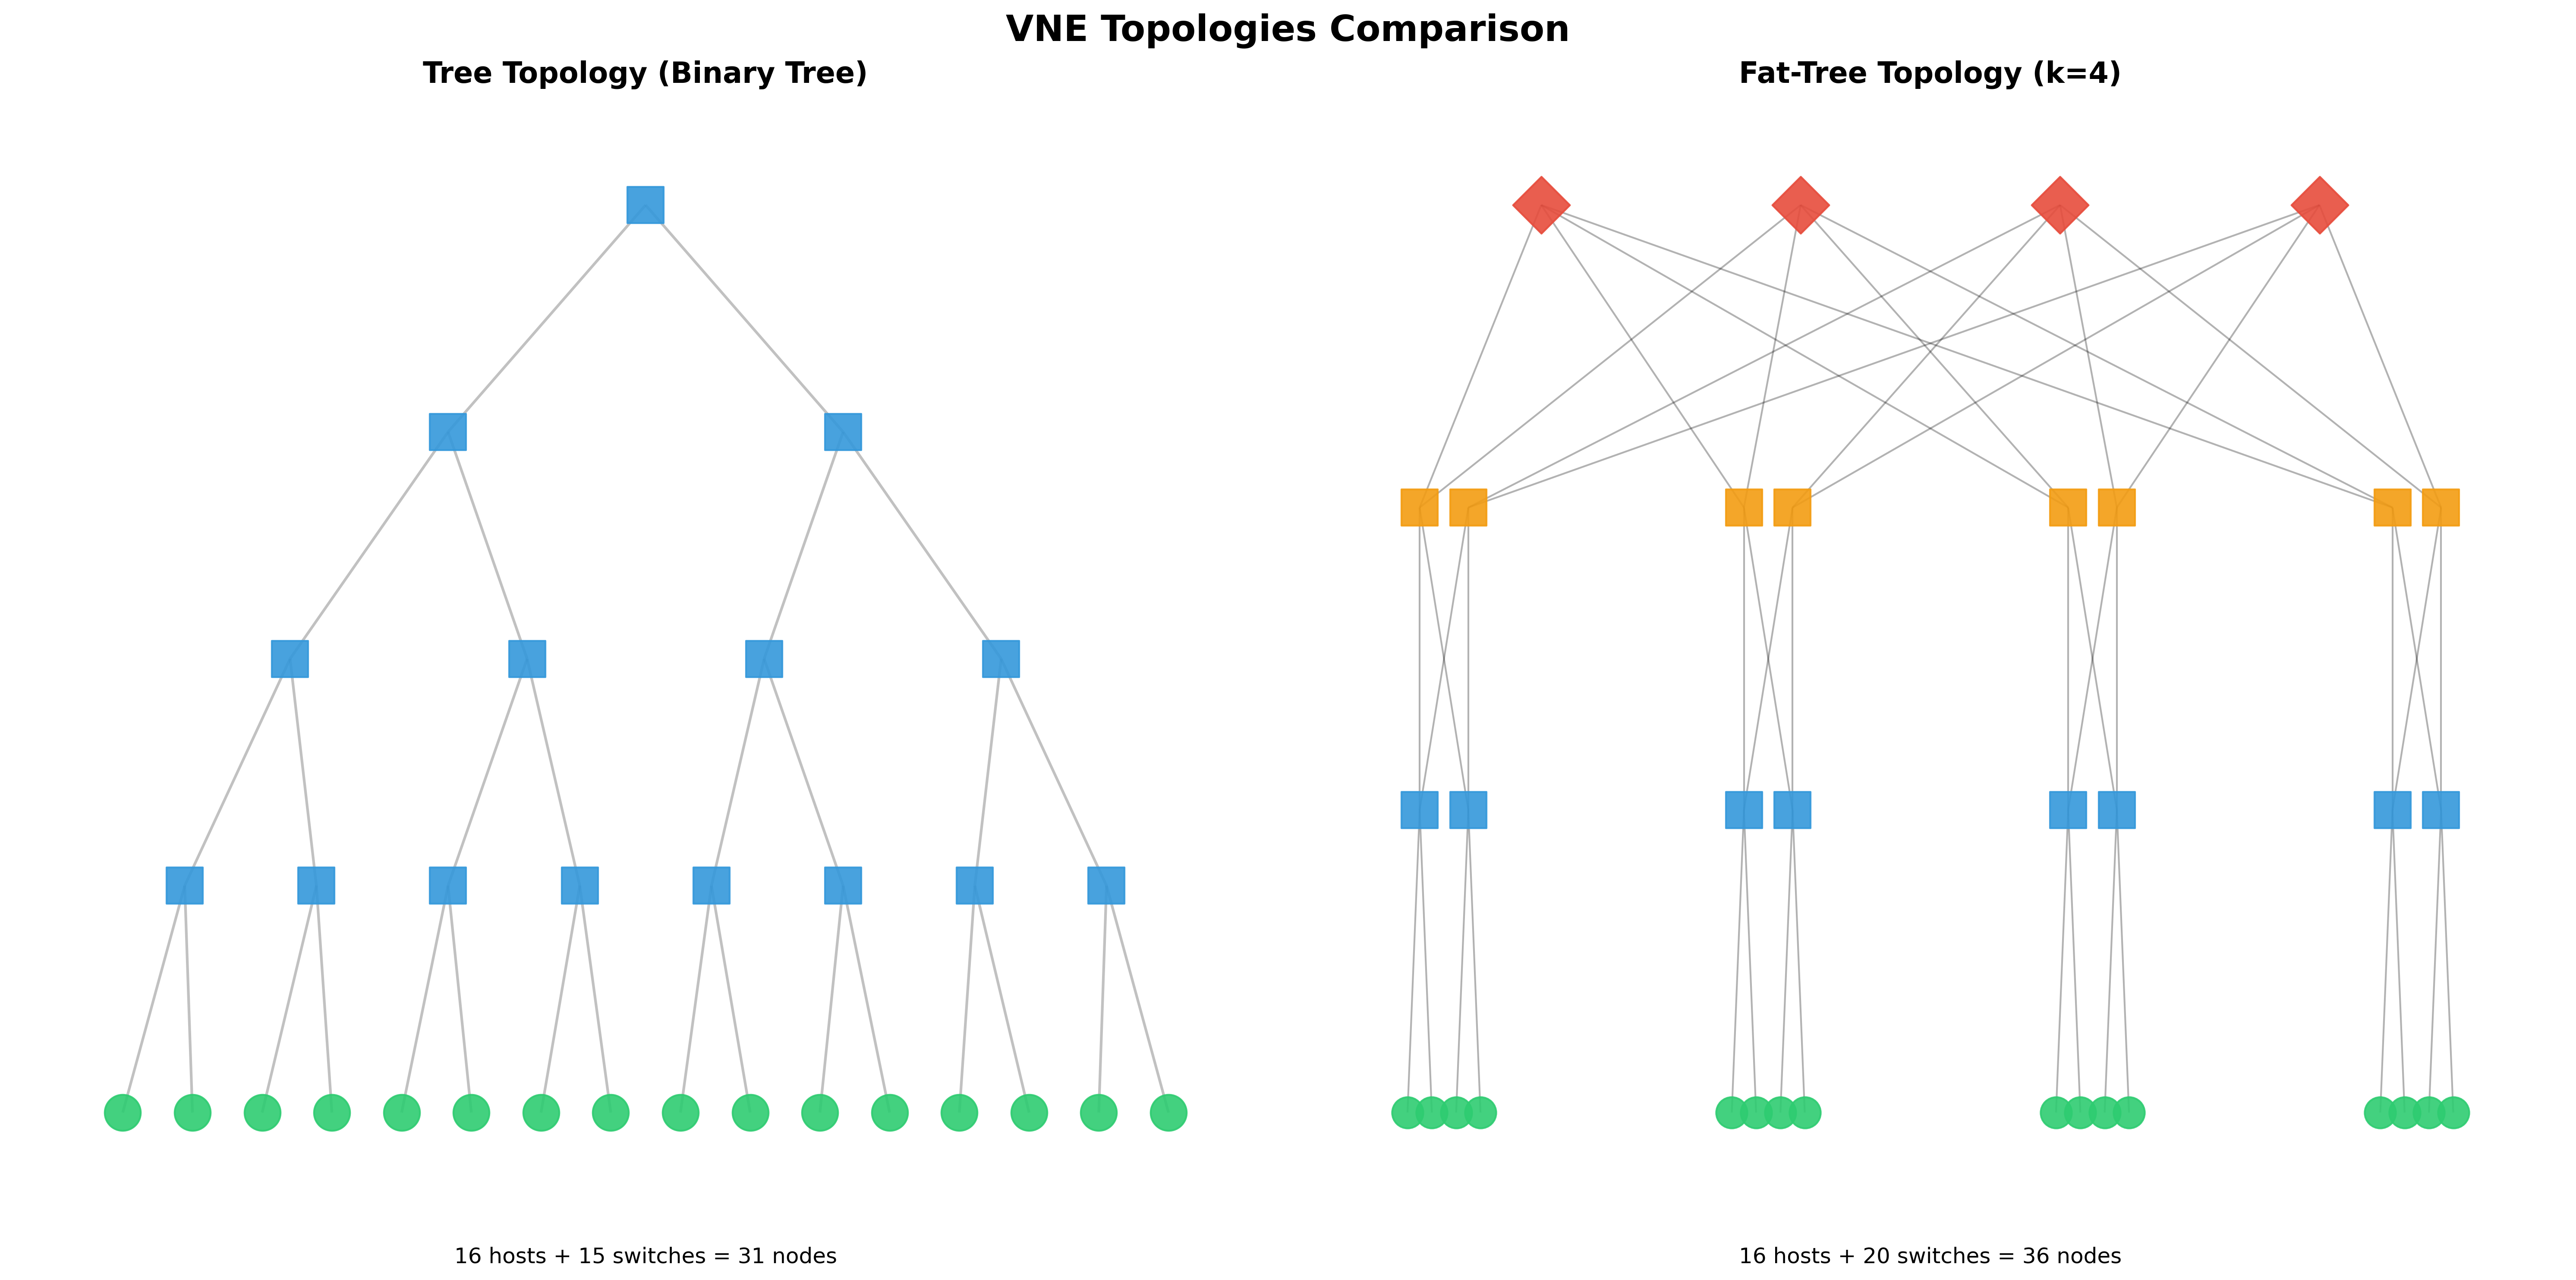
\includegraphics[width=0.95\columnwidth]{topologies_comparison}
    \caption{Comparação de Topologias: Tree (Hierárquica Binária) e Fat-Tree (\textit{Datacenter}). A topologia Tree apresenta estrutura hierárquica tradicional com hosts na base e switches em níveis sucessivos. A Fat-Tree apresenta estrutura de \textit{datacenter} com k=4, caracterizada por múltiplos caminhos e maior redundância.}
    \label{fig:topologies-comparison}
\end{figure}

A Figura~\ref{fig:waxman-topology} apresenta a terceira topologia utilizada nas simulações, a Waxman-16, que representa uma rede aleatória com características distintas das topologias estruturadas anteriores:

\begin{figure}[H]
    \centering
    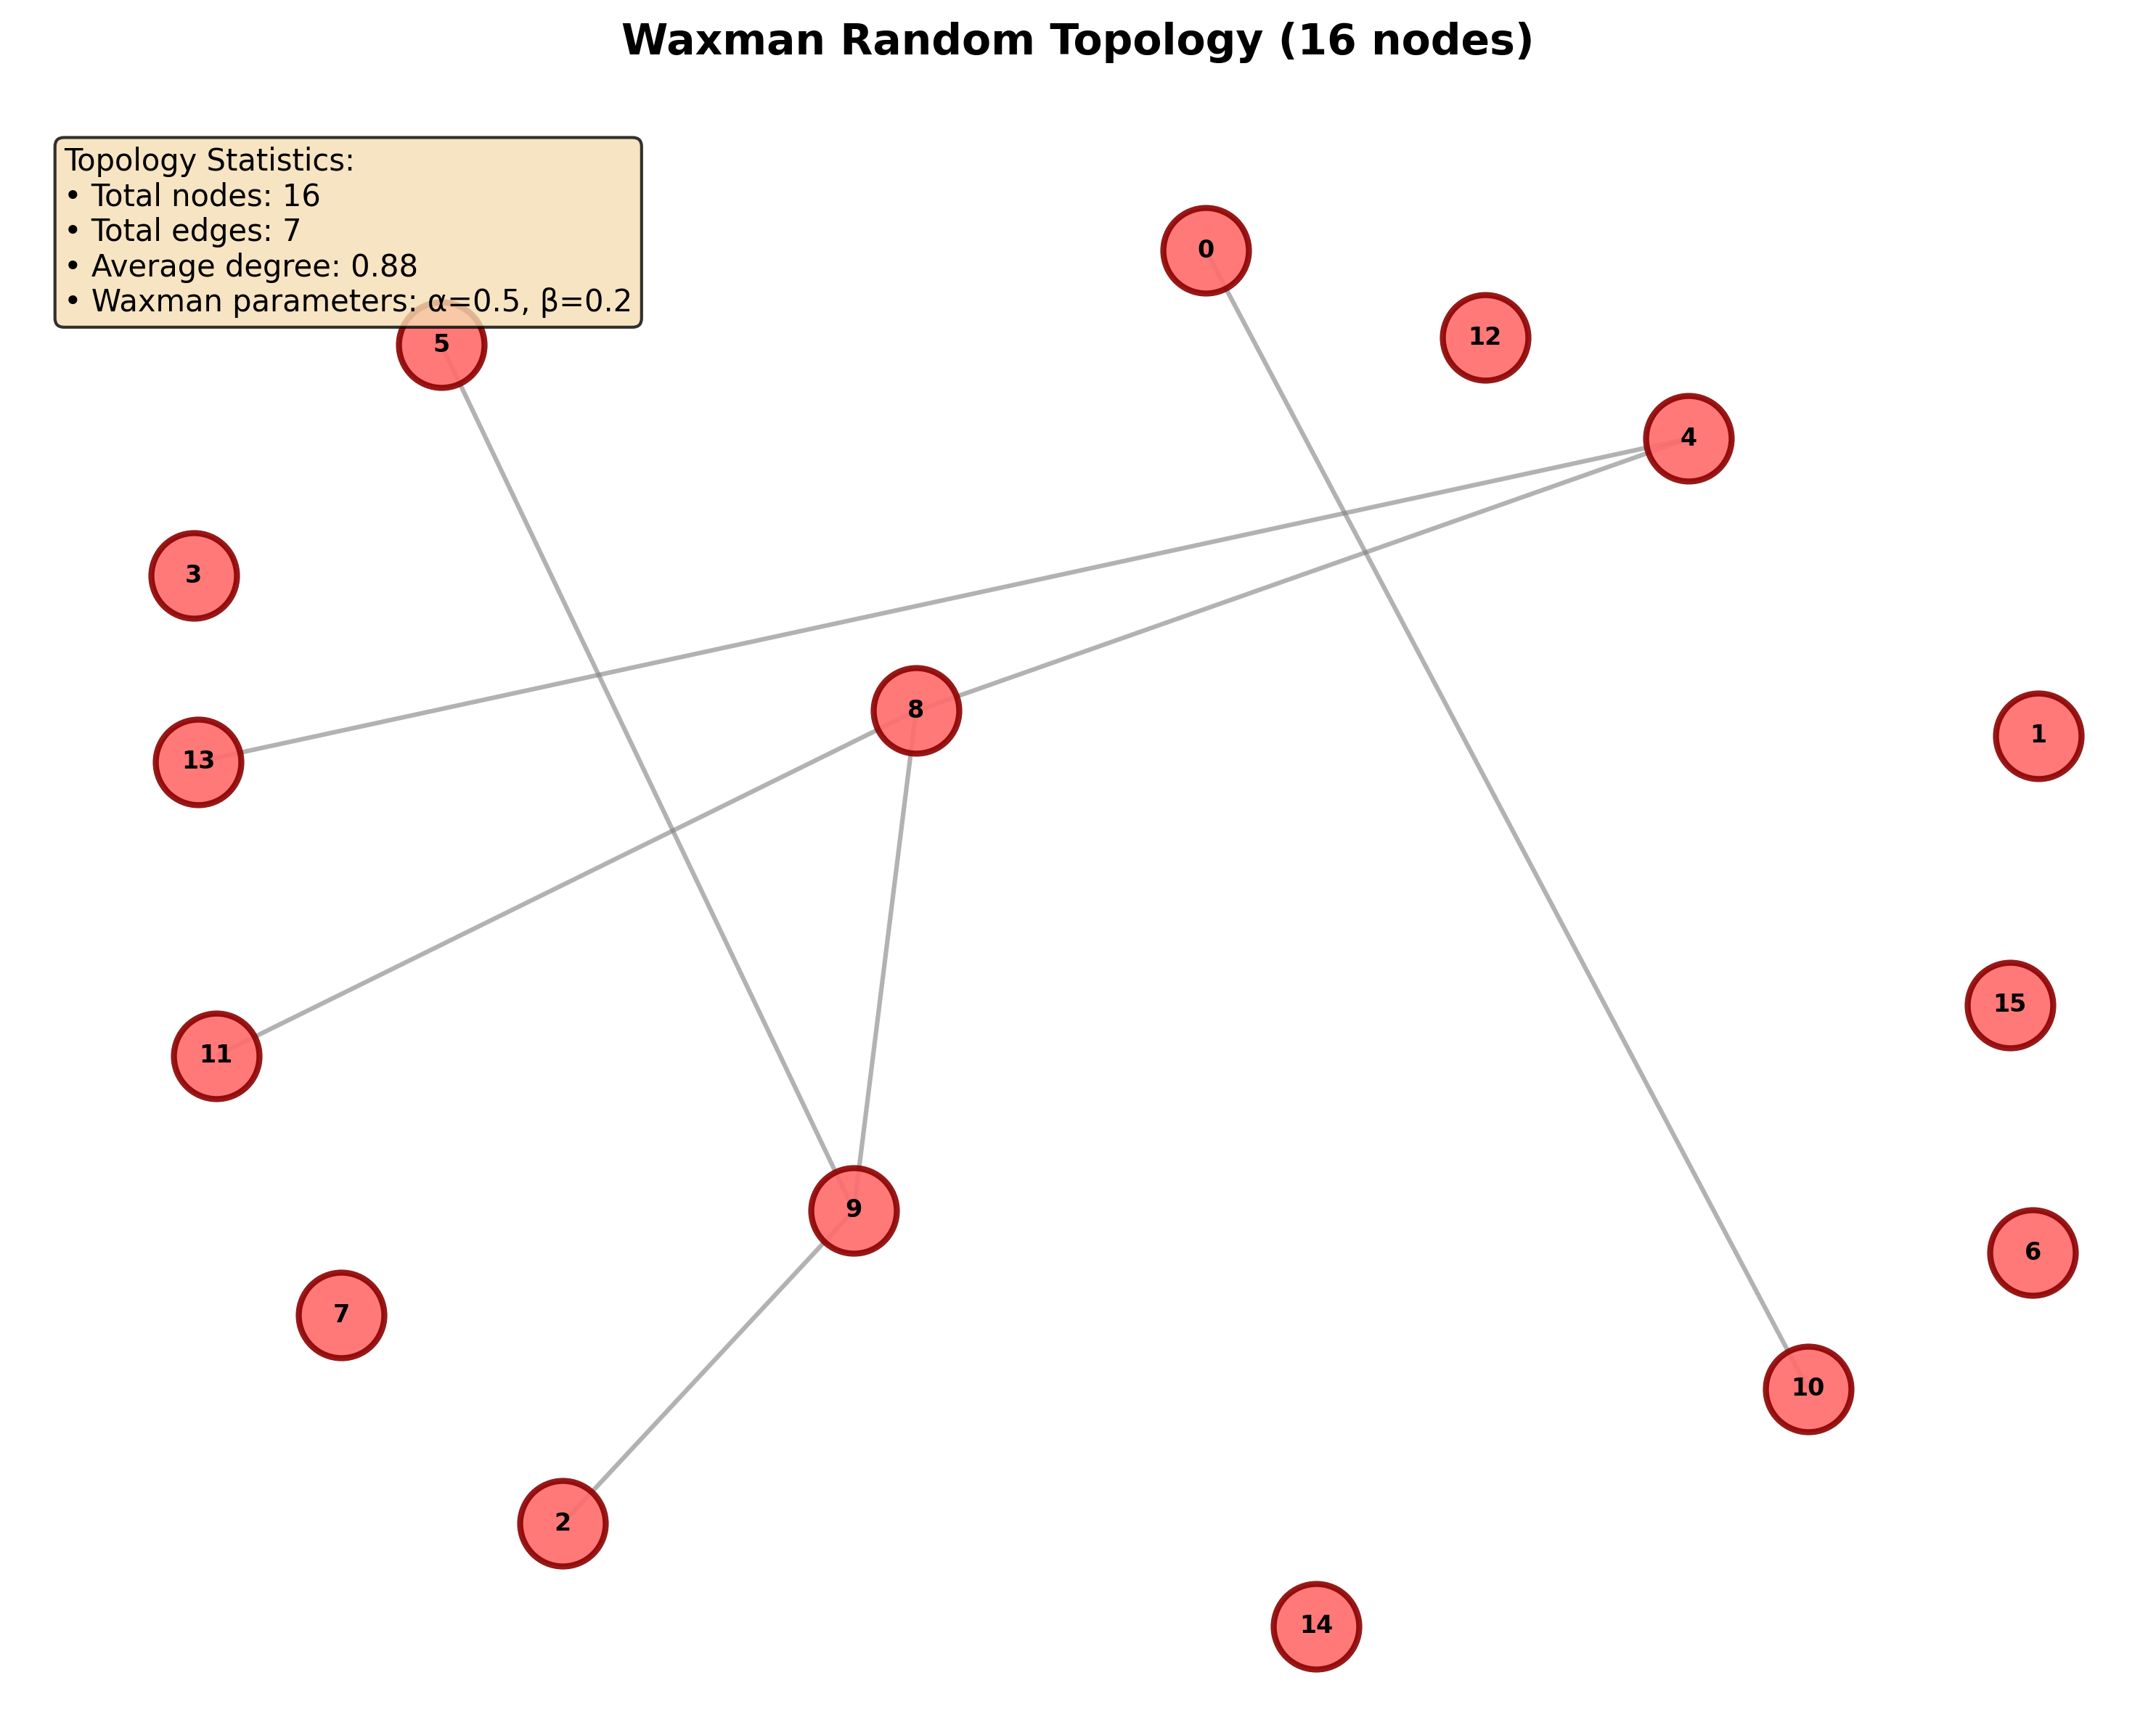
\includegraphics[width=0.7\columnwidth]{waxman_16_topology}
    \caption{Topologia Waxman-16: Rede Aleatória com 16 Nós. Diferentemente das topologias estruturadas (Tree e Fat-Tree), a Waxman representa uma rede aleatória gerada com parâmetros de dispersão geográfica ($\alpha$=0.5, $\beta$=0.2), simulando características de redes reais de larga escala, com múltiplos nós isolados e grupos conectados variáveis.}
    \label{fig:waxman-topology}
\end{figure}

\textbf{Algoritmos VNE}: MIP, GA-Meta, PSO-Meta, SA-Meta, MCTS, PL-Rank, RW-Rank-BFS, D-Round.

As simulações foram configuradas com recursos homogêneos (CPU e memória) distribuídos uniformemente nos nós físicos. As VNRs foram geradas com tamanho variável (distribuição uniforme entre 2 e 10 nós virtuais), conectividade de 50\% entre nós virtuais, e demandas de recursos seguindo distribuições realistas. O sistema simula chegadas sequenciais de VNRs com taxa de chegada segundo distribuição Poisson, em que cada requisição possui um tempo de vida estocástico. O Virne avalia automaticamente a viabilidade de cada solução proposta pelos algoritmos, verificando restrições de capacidade de nós e enlaces, e calcula métricas de desempenho padronizadas (RAC, LRC, LAR, AST) para cada execução.

Para cada combinação de algoritmo e topologia, executadas dez repetições com diferentes sementes aleatórias, totalizando aproximadamente 8000 VNRs únicos após deduplicação. Esta abordagem garante robustez estatística e captura a variabilidade inerente aos algoritmos estocásticos e às características dinâmicas das requisições de rede virtual.

\subsection{Engenharia de Features}

Um conjunto de 27 features foi cuidadosamente selecionado, dividido em categorias:

\textbf{Características da VNR} (9 features): número de nós, número de enlaces, razão de tamanho, demanda média por nó, demanda média por enlace, conectividade, demanda total, razão nó/enlace, tempo de vida esperado.

\textbf{Estado da Rede Física} (4 features): recursos disponíveis, utilização de nós, utilização de enlaces, utilização geral.

\textbf{Estado do Sistema} (3 features): número de VNRs ativas, carga do sistema, nós físicos ativos.

\textbf{Heterogeneidade e Fragmentação} (10 features engineerizados): índices de Gini para distribuição de recursos, fragmentação de memória, índices de diversidade topológica.

\textbf{Contexto} (1 feature): tipo de topologia.

\subsection{Arquitetura Multi-Objetivo}

Ao invés de um único modelo de classificação, empregamos \textbf{três modelos especializados}, cada otimizado para um objetivo específico:

\begin{itemize}
    \item \textbf{RAC}: Maximizar taxa de aceitação de requisições de rede virtual
    \item \textbf{LRC}: Maximizar razão receita-custo de longo prazo
    \item \textbf{LAR}: Maximizar receita média de longo prazo
\end{itemize}

Cada modelo é uma árvore de decisão treinada independentemente em dados históricos de simulações. Durante operação online, o operador (ou política automática) seleciona qual objetivo priorizar, e o modelo correspondente prediz o melhor algoritmo.

\subsection{Treino dos Modelos}

O processo de treinamento foi realizado de forma independente para cada objetivo (RAC, LRC, LAR), permitindo que cada modelo especialize-se na otimização de sua métrica específica. A divisão dos dados foi estratificada por classe de algoritmo para garantir distribuição balanceada entre conjuntos de treino (70\%), validação (15\%) e teste (15\%). Esta estratificação é crucial para manter representatividade de todas as classes em cada partição, especialmente considerando o desbalanceamento severo observado nos dados.

Os modelos utilizam \texttt{DecisionTreeClassifier} do scikit-learn com os seguintes hiperparâmetros otimizados:

\begin{itemize}
    \item \textbf{Profundidade máxima}: 10 (balanceando expressividade e interpretabilidade)
    \item \textbf{Mínimo de amostras por folha}: 3 (reduzido para permitir captura de classes minoritárias)
    \item \textbf{Mínimo de amostras para divisão}: 6 (permite splits com menos amostras)
    \item \textbf{Critério de divisão}: Gini (impureza de Gini para seleção de features)
\end{itemize}

Conforme mostrado na Tabela~\ref{tab:algorithm-summary}, nenhum algoritmo é universalmente ótimo, evidenciando a necessidade de seleção contextual. Esta observação justifica a abordagem de seleção dinâmica de algoritmos proposta neste trabalho.

\begin{table}[H]
\centering
\caption{Resumo de Desempenho dos Algoritmos VNE}
\label{tab:algorithm-summary}
\begin{tabular}{lcccc}
\toprule
\textbf{Algoritmo} & \textbf{Taxa Aceitação} & \textbf{Receita} & \textbf{R2C Razão} & \textbf{Tempo (s)} \\
\midrule
MIP & 36.8\% & \$186.808 & 115.6 & 1.026 \\
PL\_RANK & 29.5\% & \$388.387 & 127.4 & 0.661 \\
GA\_META & 27.9\% & \$400.628 & 139.8 & 0.603 \\
RW\_RANK\_BFS & 25.8\% & \$373.937 & 120.4 & 0.558 \\
SA\_META & 24.6\% & \$372.569 & 133.5 & 0.534 \\
MCTS & 23.9\% & \$379.748 & 167.0 & 0.468 \\
D\_ROUND & 20.4\% & \$365.430 & 246.0 & 0.357 \\
PSO\_META & 20.1\% & \$352.103 & 120.0 & 0.309 \\
\bottomrule
\end{tabular}
\end{table}

\subsection{Comparação Multi-Métrica dos Algoritmos VNE}

A seleção de algoritmos VNE não pode se basear em uma única métrica de desempenho. Diferentes contextos operacionais (alta carga, recursos limitados, requisitos de latência) exigem diferentes \textit{trade-offs}. A Figura~\ref{fig:algorithm-comparison} apresenta uma análise abrangente de quatro métricas complementares para os oito algoritmos avaliados:

\begin{figure*}[h]
    \centering
    \includegraphics[width=1.0\textwidth]{algorithm_comparison_all_metrics}
    \caption{Comparação Multi-Métrica: Taxa de Aceitação, Receita Total, Razão Receita-Custo e Tempo Médio por VNR. Os gráficos mostram distribuição de resultados em cinco execuções simuladas por algoritmo através de topologias (Tree, Fat-Tree, Waxman-16). Não existe algoritmo único que seja ótimo em todas as dimensões.}
    \label{fig:algorithm-comparison}
\end{figure*}


\subsubsection{Técnicas de Balanceamento de Classes}

Para reduzir o desbalanceamento do dataset, foram aplicadas técnicas de balanceamento de classes:

\textbf{Pesos de Classe Customizados}: Em vez do balanceamento padrão do scikit-learn, foi utilizado pesos calculados como $w_i = 1/\sqrt{f_i}$, em que $f_i$ é a frequência relativa da classe $i$. Esta estratégia atribui pesos significativamente maiores a classes raras:

\begin{itemize}
    \item Classes raras (\texttt{pso\_meta}, 17 amostras): peso 10,0$\times$
    \item Classes intermediárias (\texttt{rw\_rank\_bfs}, 39 amostras): peso 6,6$\times$
    \item Classes majoritárias (\texttt{ga\_meta}, 987 amostras): peso 1,3$\times$
\end{itemize}

\textbf{Avaliação }: Foi utilizada a métrica F1-Score ponderado e F1-Macro (média aritmética do F1 de todas as classes, tratando-as igualmente) para avaliar desempenho balanceado entre classes.

\subsection{Análise Detalhada de F1-Score por Classe}

A Tabela~\ref{tab:f1-per-class} apresenta o F1-Score por classe para o objetivo RAC, mostrando que técnicas de balanceamento permitem capturar padrões de todas as classes. Os resultados indicam que mesmo classes minoritárias, como PSO\_Meta e RW\_Rank\_BFS, apresentam F1-Score acima de 0,33, demonstrando a efetividade das técnicas de balanceamento empregadas:

\section{Resultados Experimentais}
\label{sec:Results}

\subsection{Desempenho de Classificação}

A Tabela~\ref{tab:classification-metrics} apresenta as métricas de classificação obtidas para os três objetivos considerados (RAC, LRC e LAR):

\begin{table}[H]
\centering
\caption{Métricas de Classificação por Objetivo (Modelos Balanceados)}
\label{tab:classification-metrics}
\begin{tabular}{lcccc}
\toprule
\textbf{Objetivo} & \textbf{Acurácia} & \textbf{F1-Score} & \textbf{Top-2} & \textbf{Top-3} \\
\midrule
RAC (Taxa Aceitação) & 67,26\% & 0,68 & 82,66\% & 85,90\% \\
LRC (Razão Receita-Custo) & 54,46\% & 0,55 & 74,55\% & 83,95\% \\
LAR (Receita Média) & 48,14\% & 0,48 & 67,59\% & 79,09\% \\
\bottomrule
\end{tabular}
\end{table}

Os resultados apresentados na Tabela~\ref{tab:classification-metrics} indicam que o objetivo RAC apresenta melhor desempenho em todas as métricas, com acurácia de 67,26\% e top-3 accuracy de 85,90\%. O objetivo LRC apresenta desempenho intermediário, enquanto LAR apresenta menor acurácia (48,14\%), porém ainda com top-3 accuracy de 79,09\%, indicando que o modelo frequentemente identifica o melhor algoritmo entre as três melhores opções. A diferença de desempenho entre objetivos reflete a complexidade distinta de cada métrica e a variabilidade inerente aos algoritmos em diferentes contextos.

\subsection{Comparação com \textit{Baseline}}

A acurácia da classificação foi medida para cada objetivo, comparando o desempenho da árvore de decisão com o \textit{baseline} de algoritmo fixo. A Figura~\ref{fig:baseline-comparison} apresenta os resultados. É possível perceber que a acurácia depende significativamente do algoritmo fixo escolhido, evidenciando a necessidade de seleção contextual.

\begin{figure}[H]
\centering

\includegraphics[width=0.95\columnwidth]{baseline_comparison_chart}
\caption{Comparação de Acurácia: Baseline vs Árvore de Decisão por Objetivo de Otimização}
\label{fig:baseline-comparison}
\end{figure}

A Figura~\ref{fig:baseline-comparison} revela que a seleção contextual via árvores de decisão supera significativamente o uso de algoritmos fixos. Para o objetivo RAC, a melhoria é de +32,90 pontos percentuais (+95,8\% relativo), enquanto para LRC e LAR as melhorias são ainda mais expressivas em termos relativos (+100,0\% e +110,7\%, respectivamente). Estes resultados confirmam que a seleção adaptativa de algoritmos baseada em características contextuais é fundamental para otimizar o desempenho do sistema.

Para validar que os ganhos em acurácia de classificação se traduzem em melhoria de desempenho operacional real, foi avaliado o desempenho quando as árvores de decisão são utilizadas para seleção de algoritmos em execuções simuladas. 
A Figura~\ref{fig:real-performance-improvement} apresenta a comparação do desempenho real (usando valores individuais por VNR) entre seleção via árvore e \textit{baseline} de algoritmo fixo.

\begin{figure}[H]
\centering
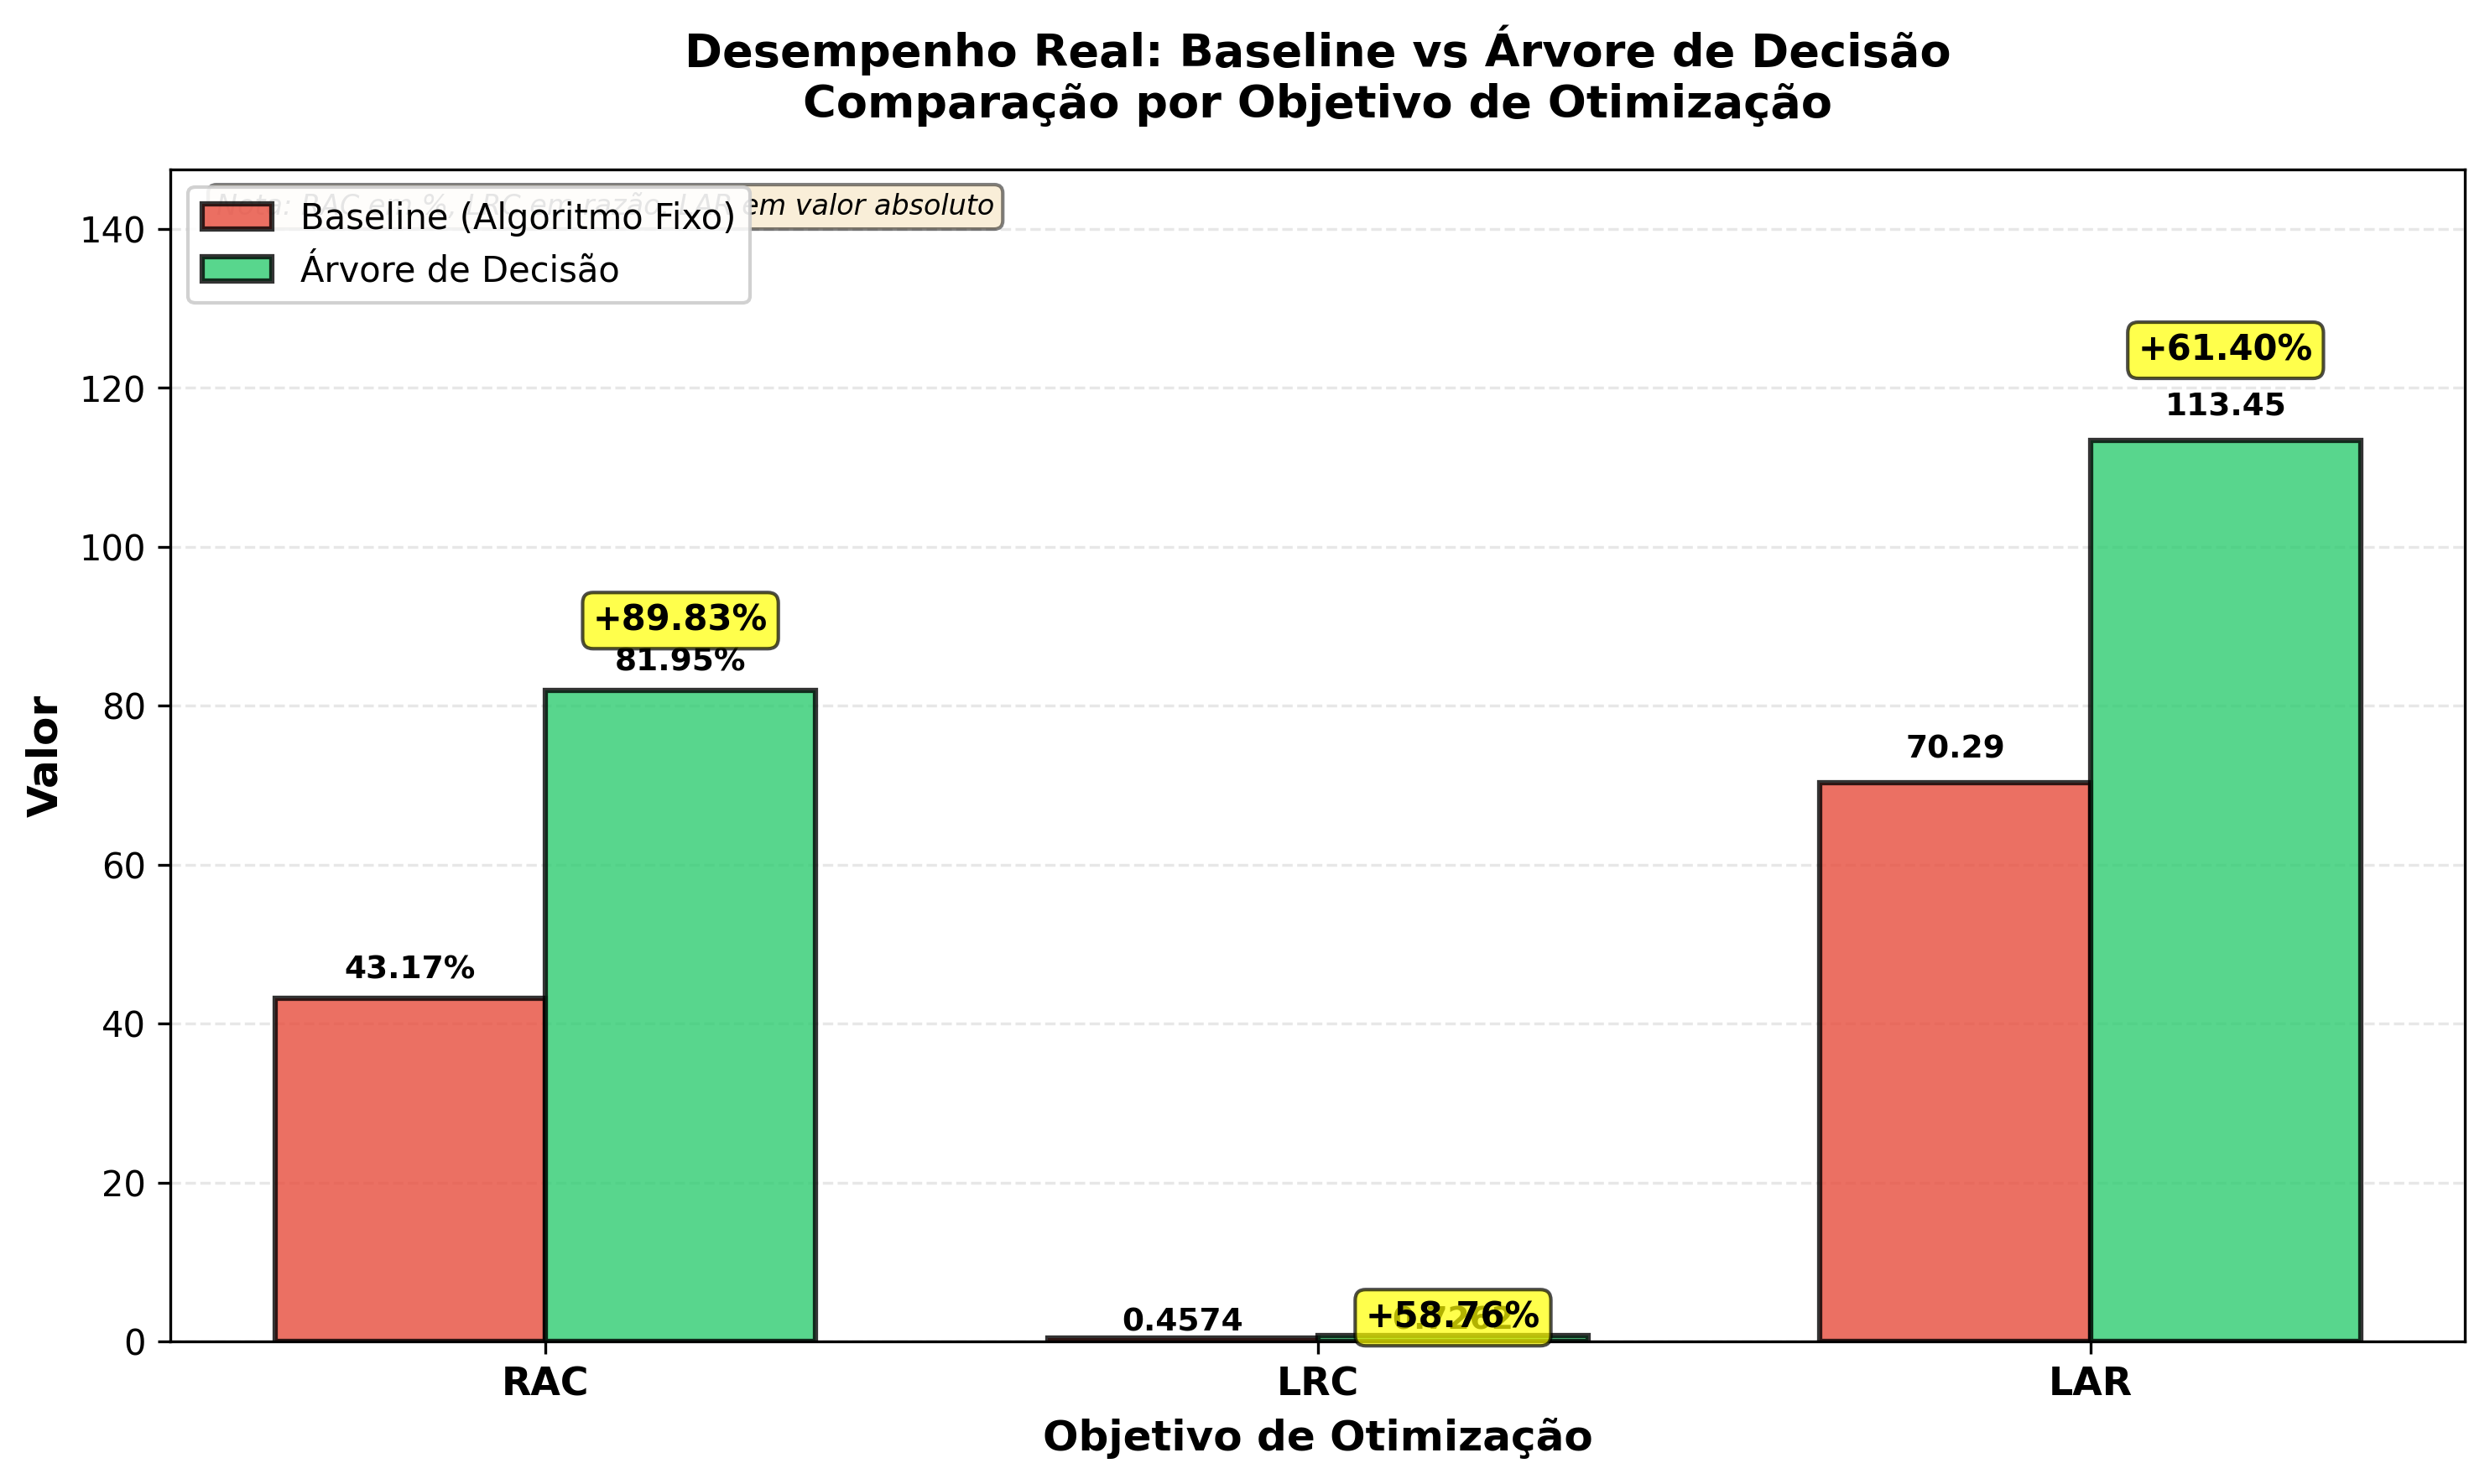
\includegraphics[width=0.95\columnwidth]{real_performance_chart}
\caption{Desempenho Real: Árvore vs Baseline por Objetivo de Otimização}
\label{fig:real-performance-improvement}
\end{figure}

A Figura~\ref{fig:real-performance-improvement} apresenta os resultados de desempenho operacional real quando as árvores de decisão são utilizadas para seleção de algoritmos. Os resultados mostram que a seleção contextual via árvores de decisão produz \textbf{melhorias substanciais de desempenho operacional real} em todos os objetivos:

\begin{itemize}
    \item \textbf{RAC}: Taxa de aceitação aumenta de 43,17\% (algoritmo fixo) para 81,95\% (seleção contextual), representando melhoria de \textbf{+89,83\%}
    \item \textbf{LRC}: Razão receita-custo aumenta de 0,4574 para 0,7262, com melhoria de \textbf{+58,76\%}
    \item \textbf{LAR}: Receita média aumenta de 70,29 para 113,45 por VNR, com melhoria de \textbf{+61,40\%}
\end{itemize}

Os resultados mostram que a seleção contextual via árvores de decisão é significativamente superior ao uso de um algoritmo fixo, com melhorias substanciais em todos os objetivos avaliados. A abordagem captura padrões importantes de seleção de algoritmos baseados nas características contextuais das VNRs, permitindo adaptação dinâmica às diferentes condições de rede e requisitos de recursos.

A análise revela padrões importantes:

\textbf{Nenhum Algoritmo é Universalmente Ótimo}: MIP maximiza taxa de aceitação (36,8\%), GA\_META maximiza receita (400.628), D\_ROUND oferece melhor razão custo-benefício (246,0) e PSO\_META é mais rápido (0,31s). Cada algoritmo excele em uma dimensão diferente.

\textbf{Trade-offs Explícitos}: MIP oferece alta aceitação mas com tempo de processamento elevado (1,03s). D\_ROUND é muito rápido mas com aceitação reduzida (20,4\%). GA\_META oferece equilíbrio adequado entre receita e tempo de processamento.

\textbf{Justificativa para Abordagem Multi-Objetivo}: Esta variação de desempenho evidencia empiricamente que:
\begin{itemize}
    \item Algoritmo fixo único não pode servir todos os contextos operacionais
    \item Seleção contextual baseada em estado da rede e características da VNR é essencial
    \item Árvores de decisão multi-objetivo aprendem a mapear contexto $\rightarrow$ algoritmo apropriado
    \item Sistema pode adaptar prioridades em tempo de execução (aceitação vs receita vs tempo de processamento)
\end{itemize}

A Tabela~\ref{tab:algorithm-summary} sintetiza métricas agregadas para referência.

\begin{table}[H]
\centering
\caption{F1-Score por Classe - Objetivo RAC (Modelos Balanceados)}
\label{tab:f1-per-class}
\begin{tabular}{lccc}
\toprule
\textbf{Algoritmo} & \textbf{Precisão} & \textbf{Recall} & \textbf{F1-Score} \\
\midrule
GA\_Meta & 0,73 & 0,74 & 0,73 \\
MCTS & 0,78 & 0,72 & 0,75 \\
PL\_Rank & 0,77 & 0,66 & 0,71 \\
D\_Round & 0,61 & 0,59 & 0,60 \\
MIP & 0,49 & 0,57 & 0,53 \\
SA\_Meta & 0,43 & 0,56 & 0,49 \\
RW\_Rank\_BFS & 0,67 & 0,25 & 0,36 \\
PSO\_Meta & 0,22 & 0,67 & 0,33 \\
\midrule
\textbf{F1-Macro} & \multicolumn{3}{c}{\textbf{0,56}} \\
\textbf{F1-Ponderado} & \multicolumn{3}{c}{\textbf{0,68}} \\
\bottomrule
\end{tabular}
\end{table}

A análise detalhada apresentada na Tabela~\ref{tab:f1-per-class} revela que as técnicas de balanceamento permitem capturar padrões mesmo de classes minoritárias. Algoritmos como GA\_Meta, MCTS e PL\_Rank apresentam F1-Score acima de 0,70, indicando boa capacidade de predição. Classes minoritárias como PSO\_Meta e RW\_Rank\_BFS apresentam F1-Score mais baixo (0,33 e 0,36, respectivamente), porém ainda acima de zero, demonstrando que o modelo consegue identificar padrões mesmo para estas classes. O F1-Macro de 0,56 e F1-Ponderado de 0,68 indicam que o modelo apresenta desempenho balanceado entre todas as classes, com maior peso nas classes mais frequentes.

\subsection{Análise de Interpretabilidade}

Uma das principais vantagens da abordagem é que cada decisão pode ser rastreada através da árvore de decisão. A Figura~\ref{fig:decision-tree-example} mostra um fragmento simplificado de uma árvore, ilustrando como o modelo classifica VNRs:

\begin{figure}[H]
    \centering
    
\includegraphics[width=0.8\columnwidth]{tree_visualization_example}
    \caption{Exemplo de Caminho de Decisão em Árvore}
    \label{fig:decision-tree-example}
\end{figure}

Diferentemente de redes neurais profundas (caixa preta), operadores podem compreender \textbf{exatamente por que} um algoritmo foi selecionado:

\textit{``Se tamanho da VNR $<$ 30\% da rede física E utilização de nós $>$ 70\%, então selecione MIP (exato, aceita em congestionamento). Caso contrário, se conectividade $>$ 0.5, selecione GA-Meta.''}

Além disso, a análise de importância de features revela quais características são mais relevantes para cada objetivo. Para RAC (Request Acceptance Rate) e LRC (Long-Term Revenue-to-Cost), a eficiência de recursos ($resource\_efficiency$) é a feature mais crítica, com importância de 0,13 e 0,11 respectivamente. No caso de LAR (Long-Term Average Revenue), a demanda por link da VNR ($v\_net\_demand\_per\_link$) e a demanda total ($v\_net\_total\_demand$) são as features dominantes. Essas descobertas confirmam que diferentes objetivos priorizam características distintas das VNRs e do estado da rede física. A Figura~\ref{fig:feature-importance-rac} exemplifica a importância das features para o objetivo RAC, enquanto as Figuras~\ref{fig:feature-importance-lrc} e~\ref{fig:feature-importance-lar} apresentam os resultados para os demais objetivos.

\begin{figure}[H]
    \centering
    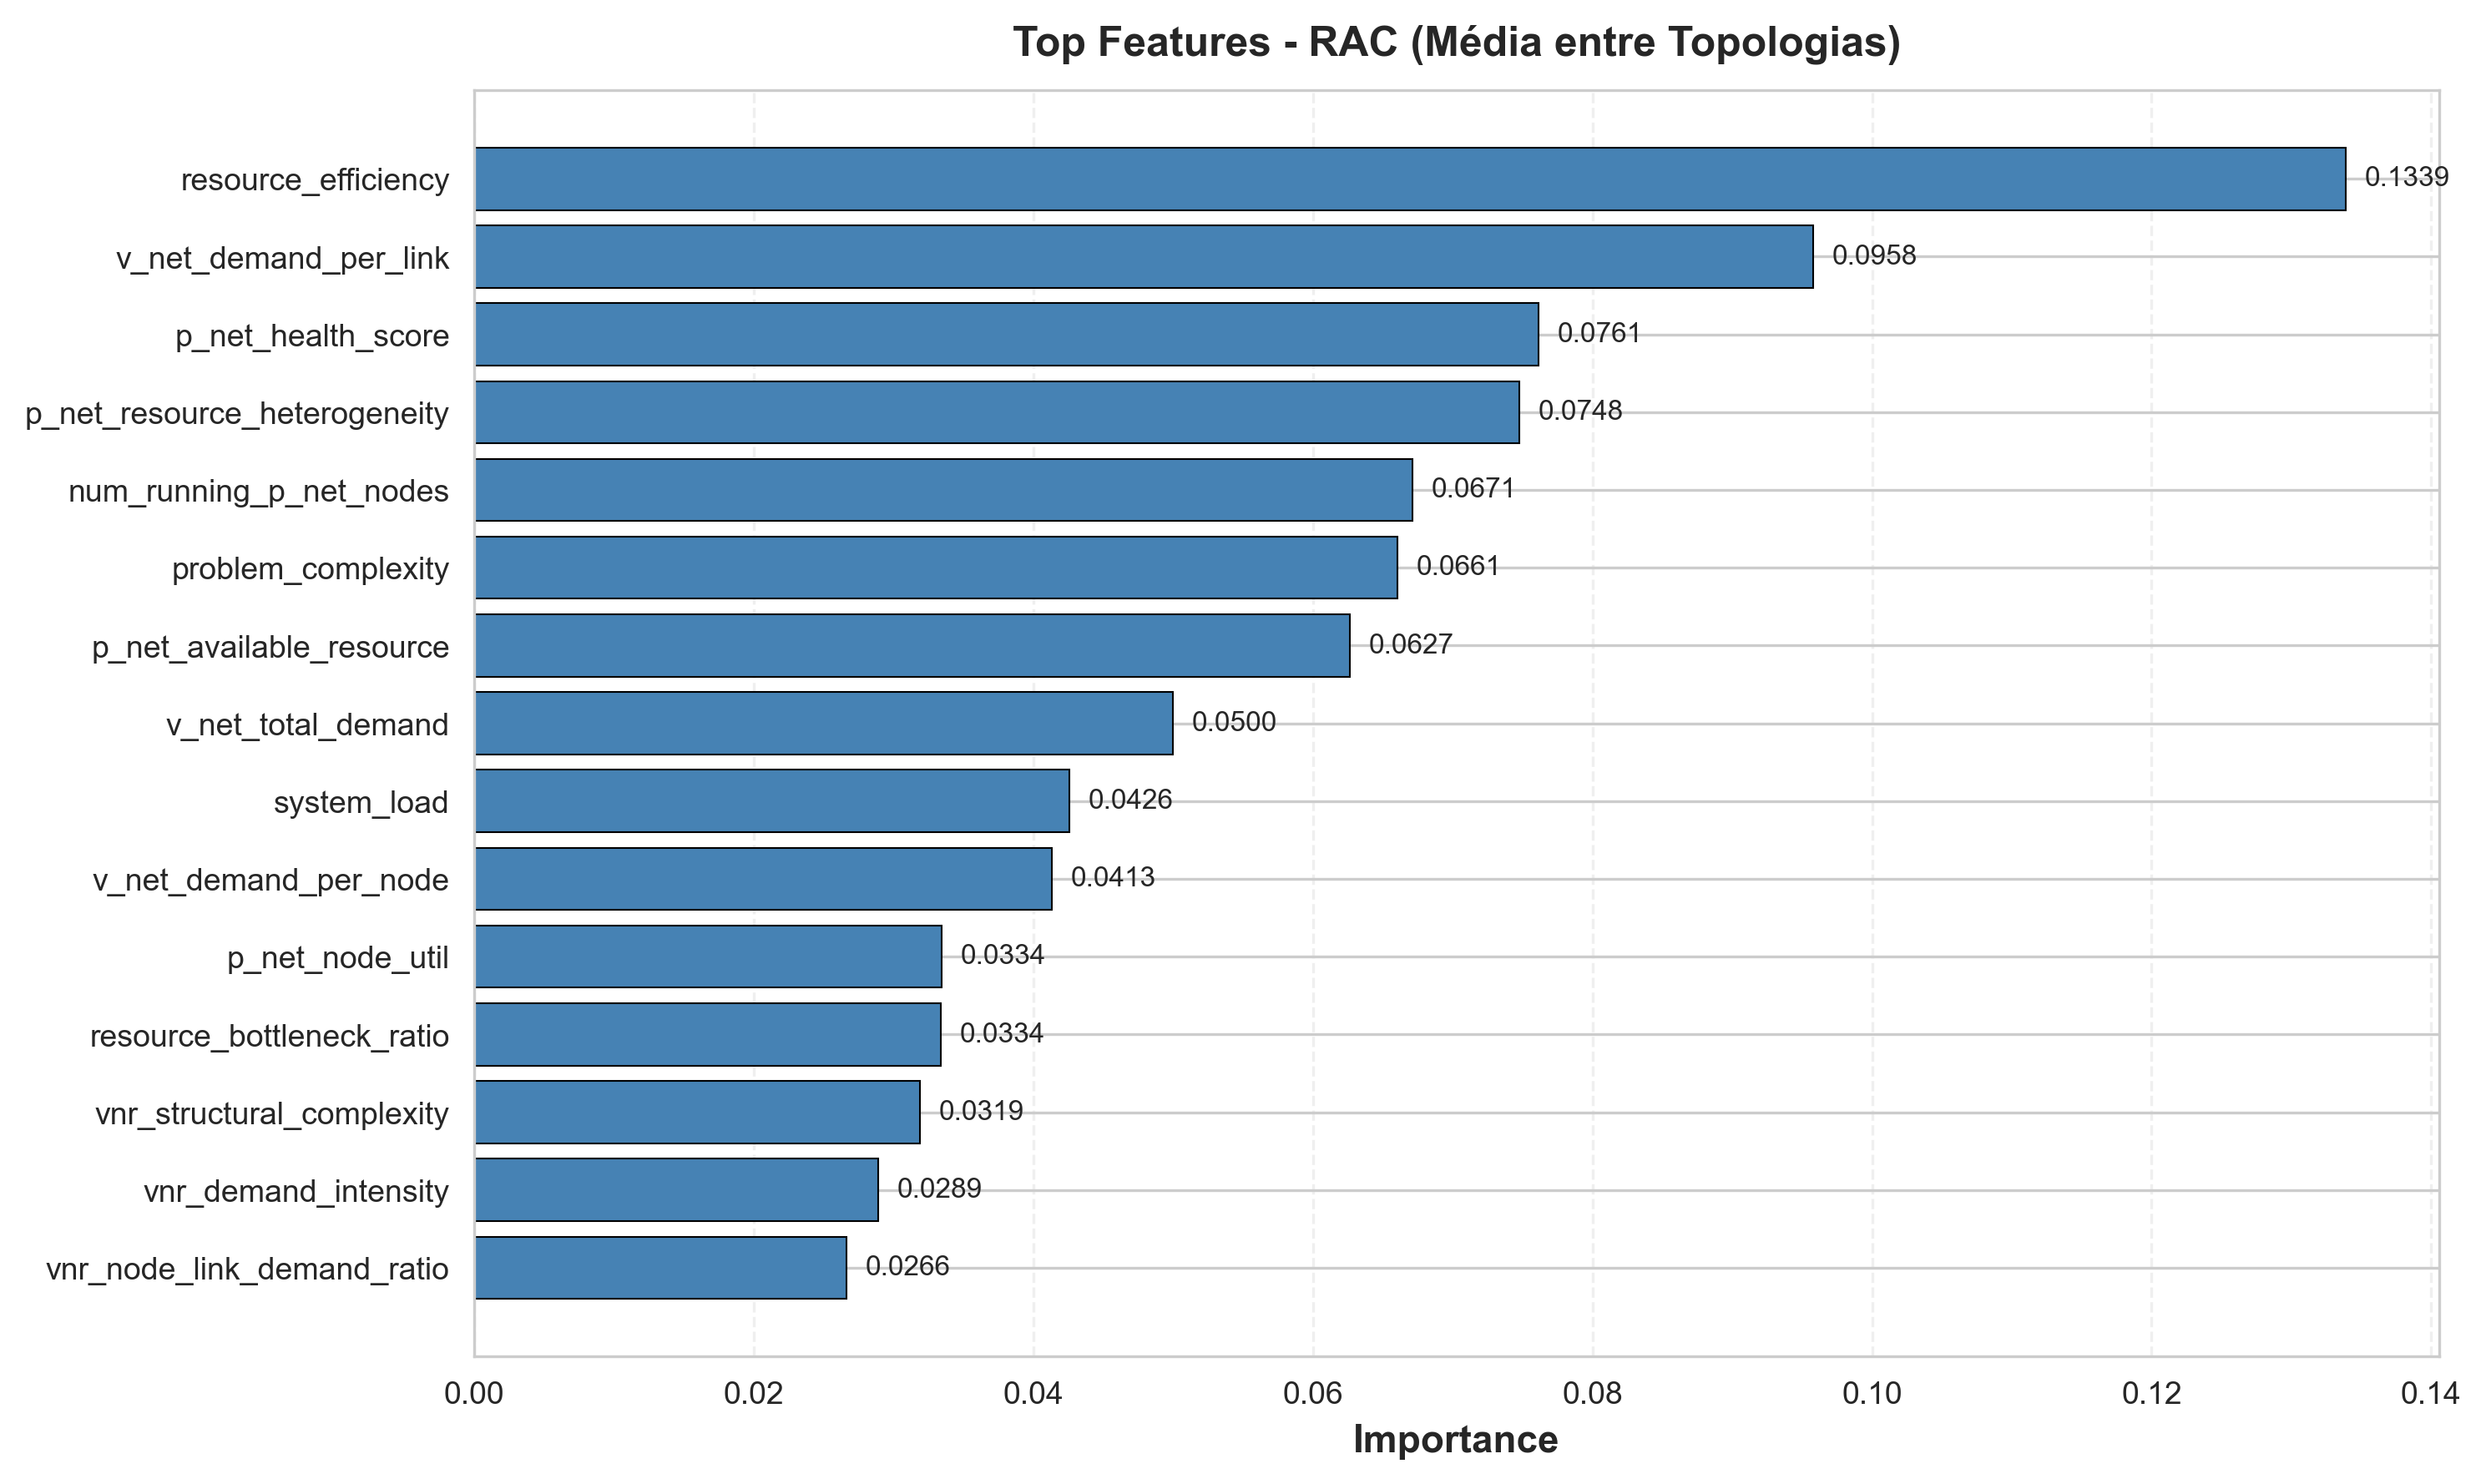
\includegraphics[width=0.95\columnwidth]{per_objective_rac}
    \caption{Importância de Features - RAC (Request Acceptance Rate). As top 15 features mais importantes (média entre topologias) para o objetivo RAC. A eficiência de recursos ($resource\_efficiency$) é a feature mais crítica com importância de 0,134, seguida pela demanda por link da VNR ($v\_net\_demand\_per\_link$) com 0,096.}
    \label{fig:feature-importance-rac}
\end{figure}

\begin{figure}[H]
    \centering
    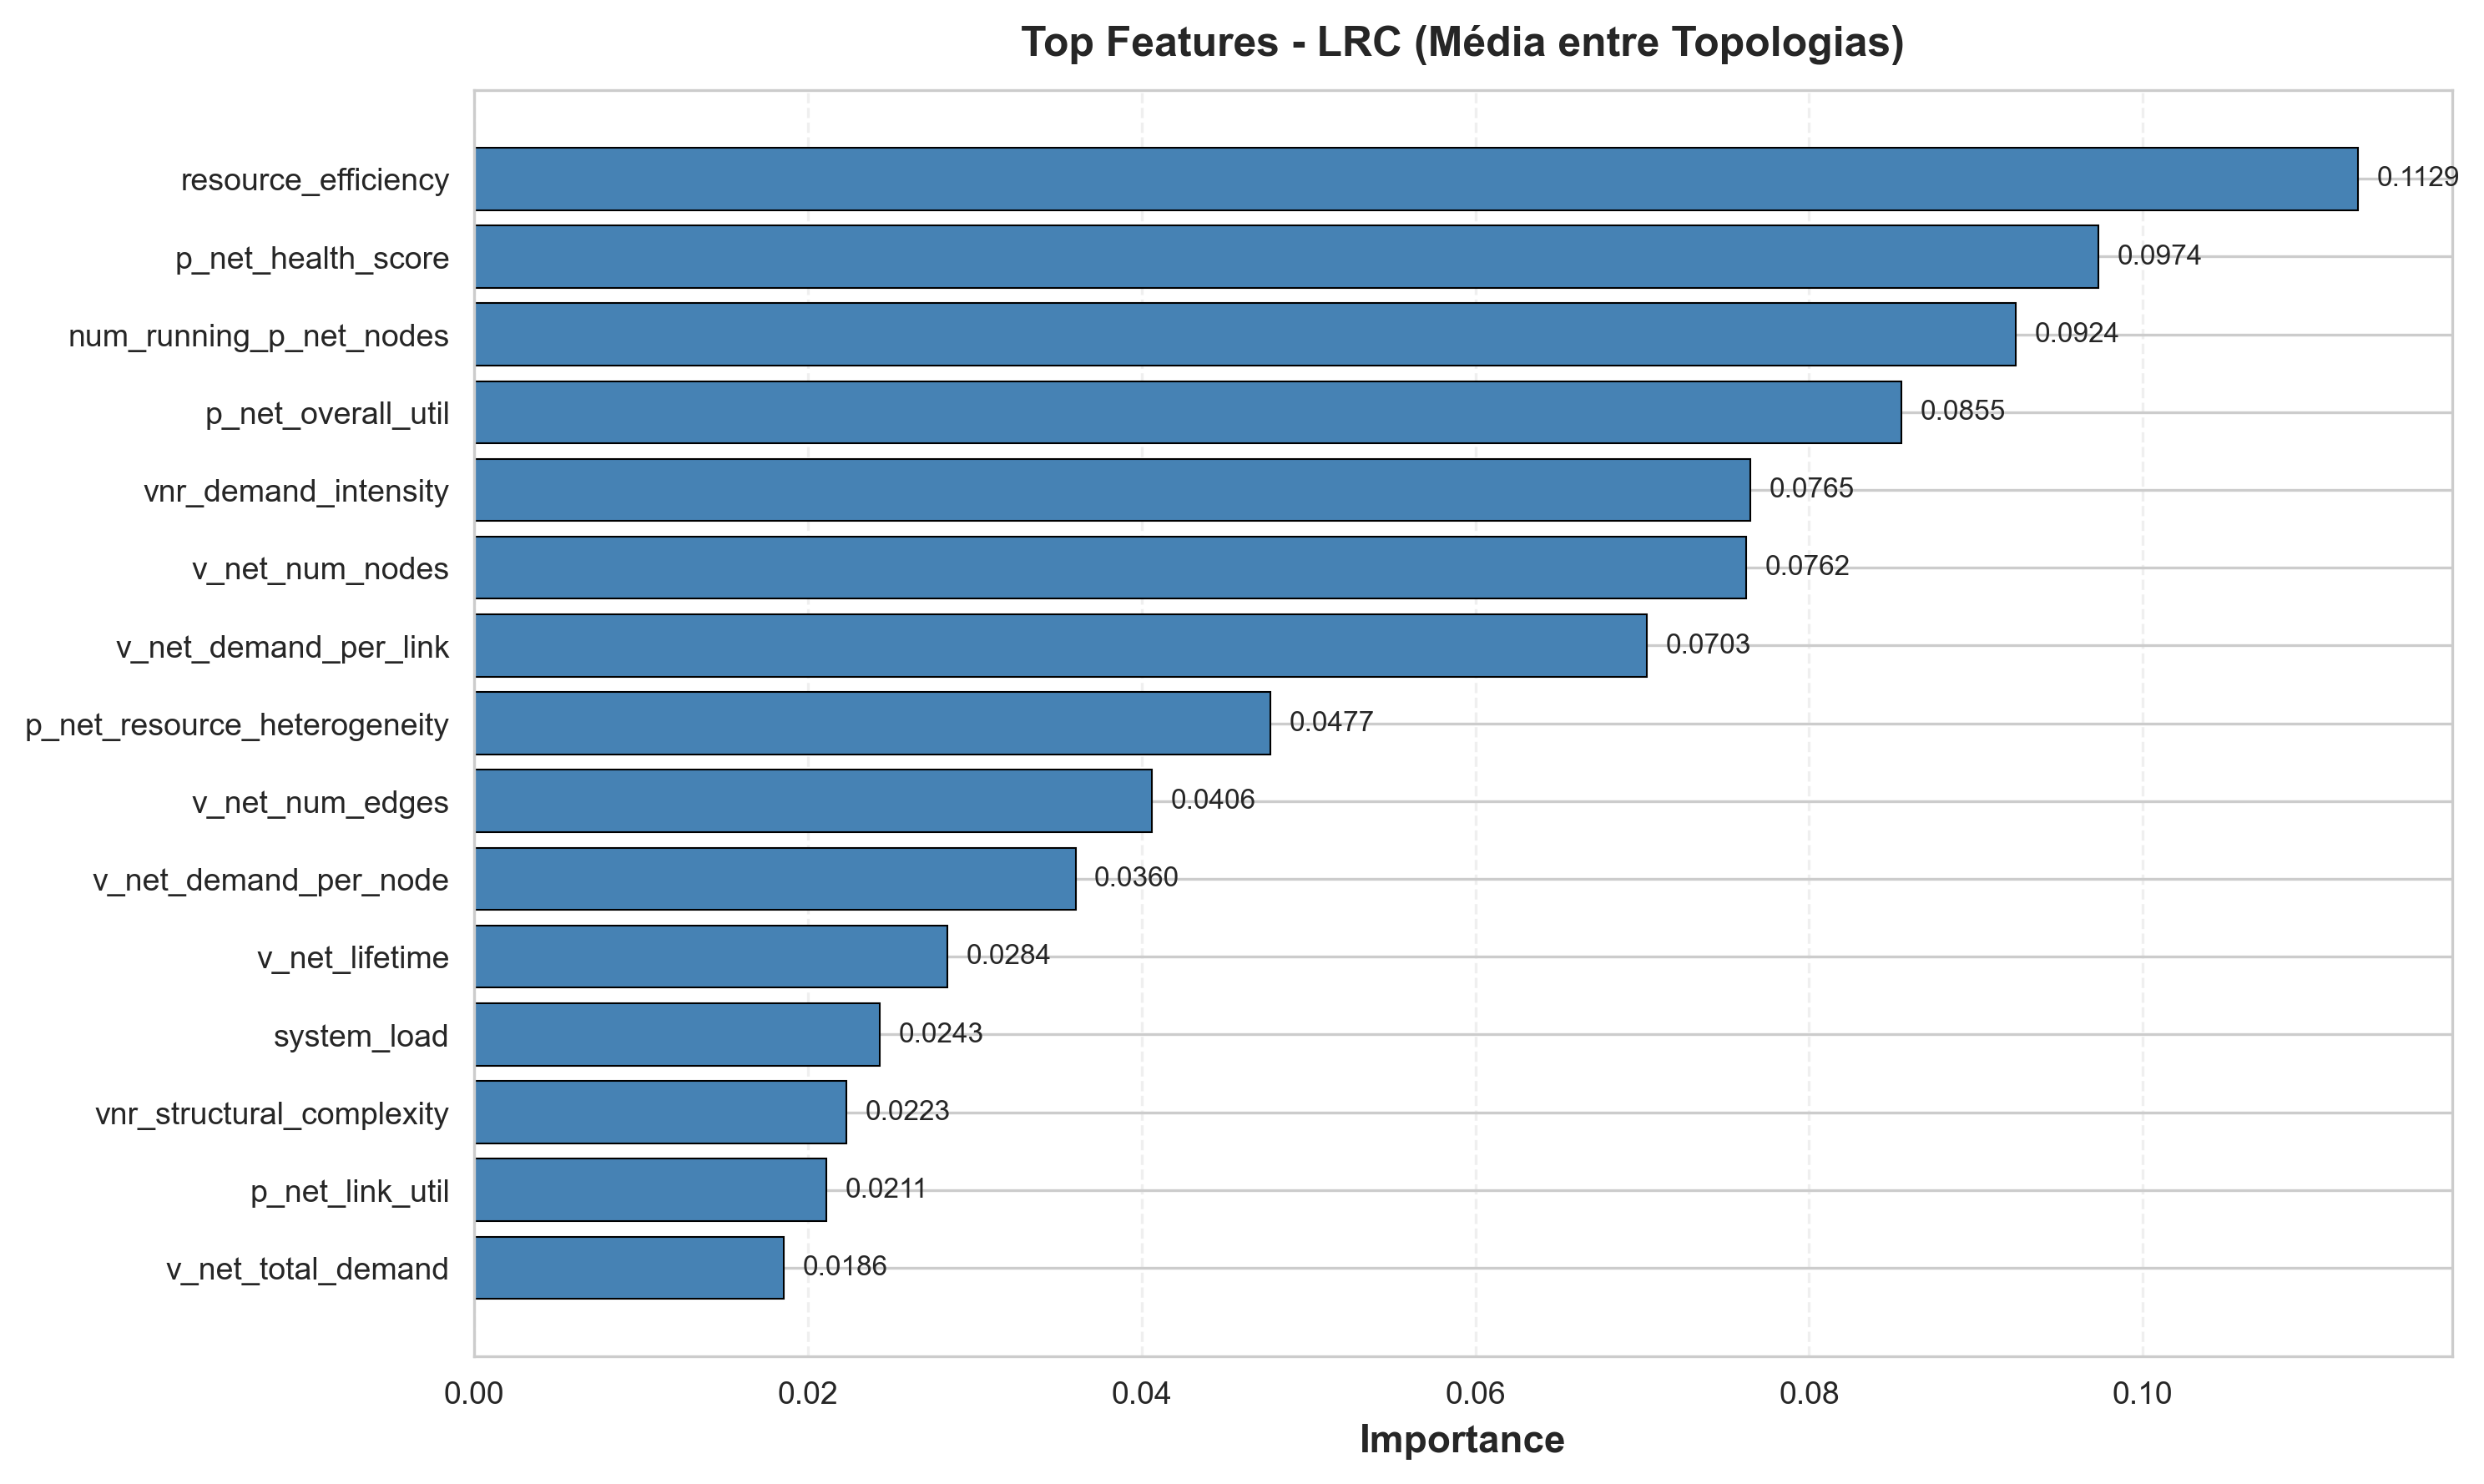
\includegraphics[width=0.95\columnwidth]{per_objective_lrc}
    \caption{Importância de Features - LRC (Long-Term Revenue-to-Cost). As top 15 features mais importantes (média entre topologias) para o objetivo LRC. A eficiência de recursos ($resource\_efficiency$) é a feature mais crítica com importância de 0,113, seguida pela saúde da rede física ($p\_net\_health\_score$) com 0,097.}
    \label{fig:feature-importance-lrc}
\end{figure}

\begin{figure}[H]
    \centering
    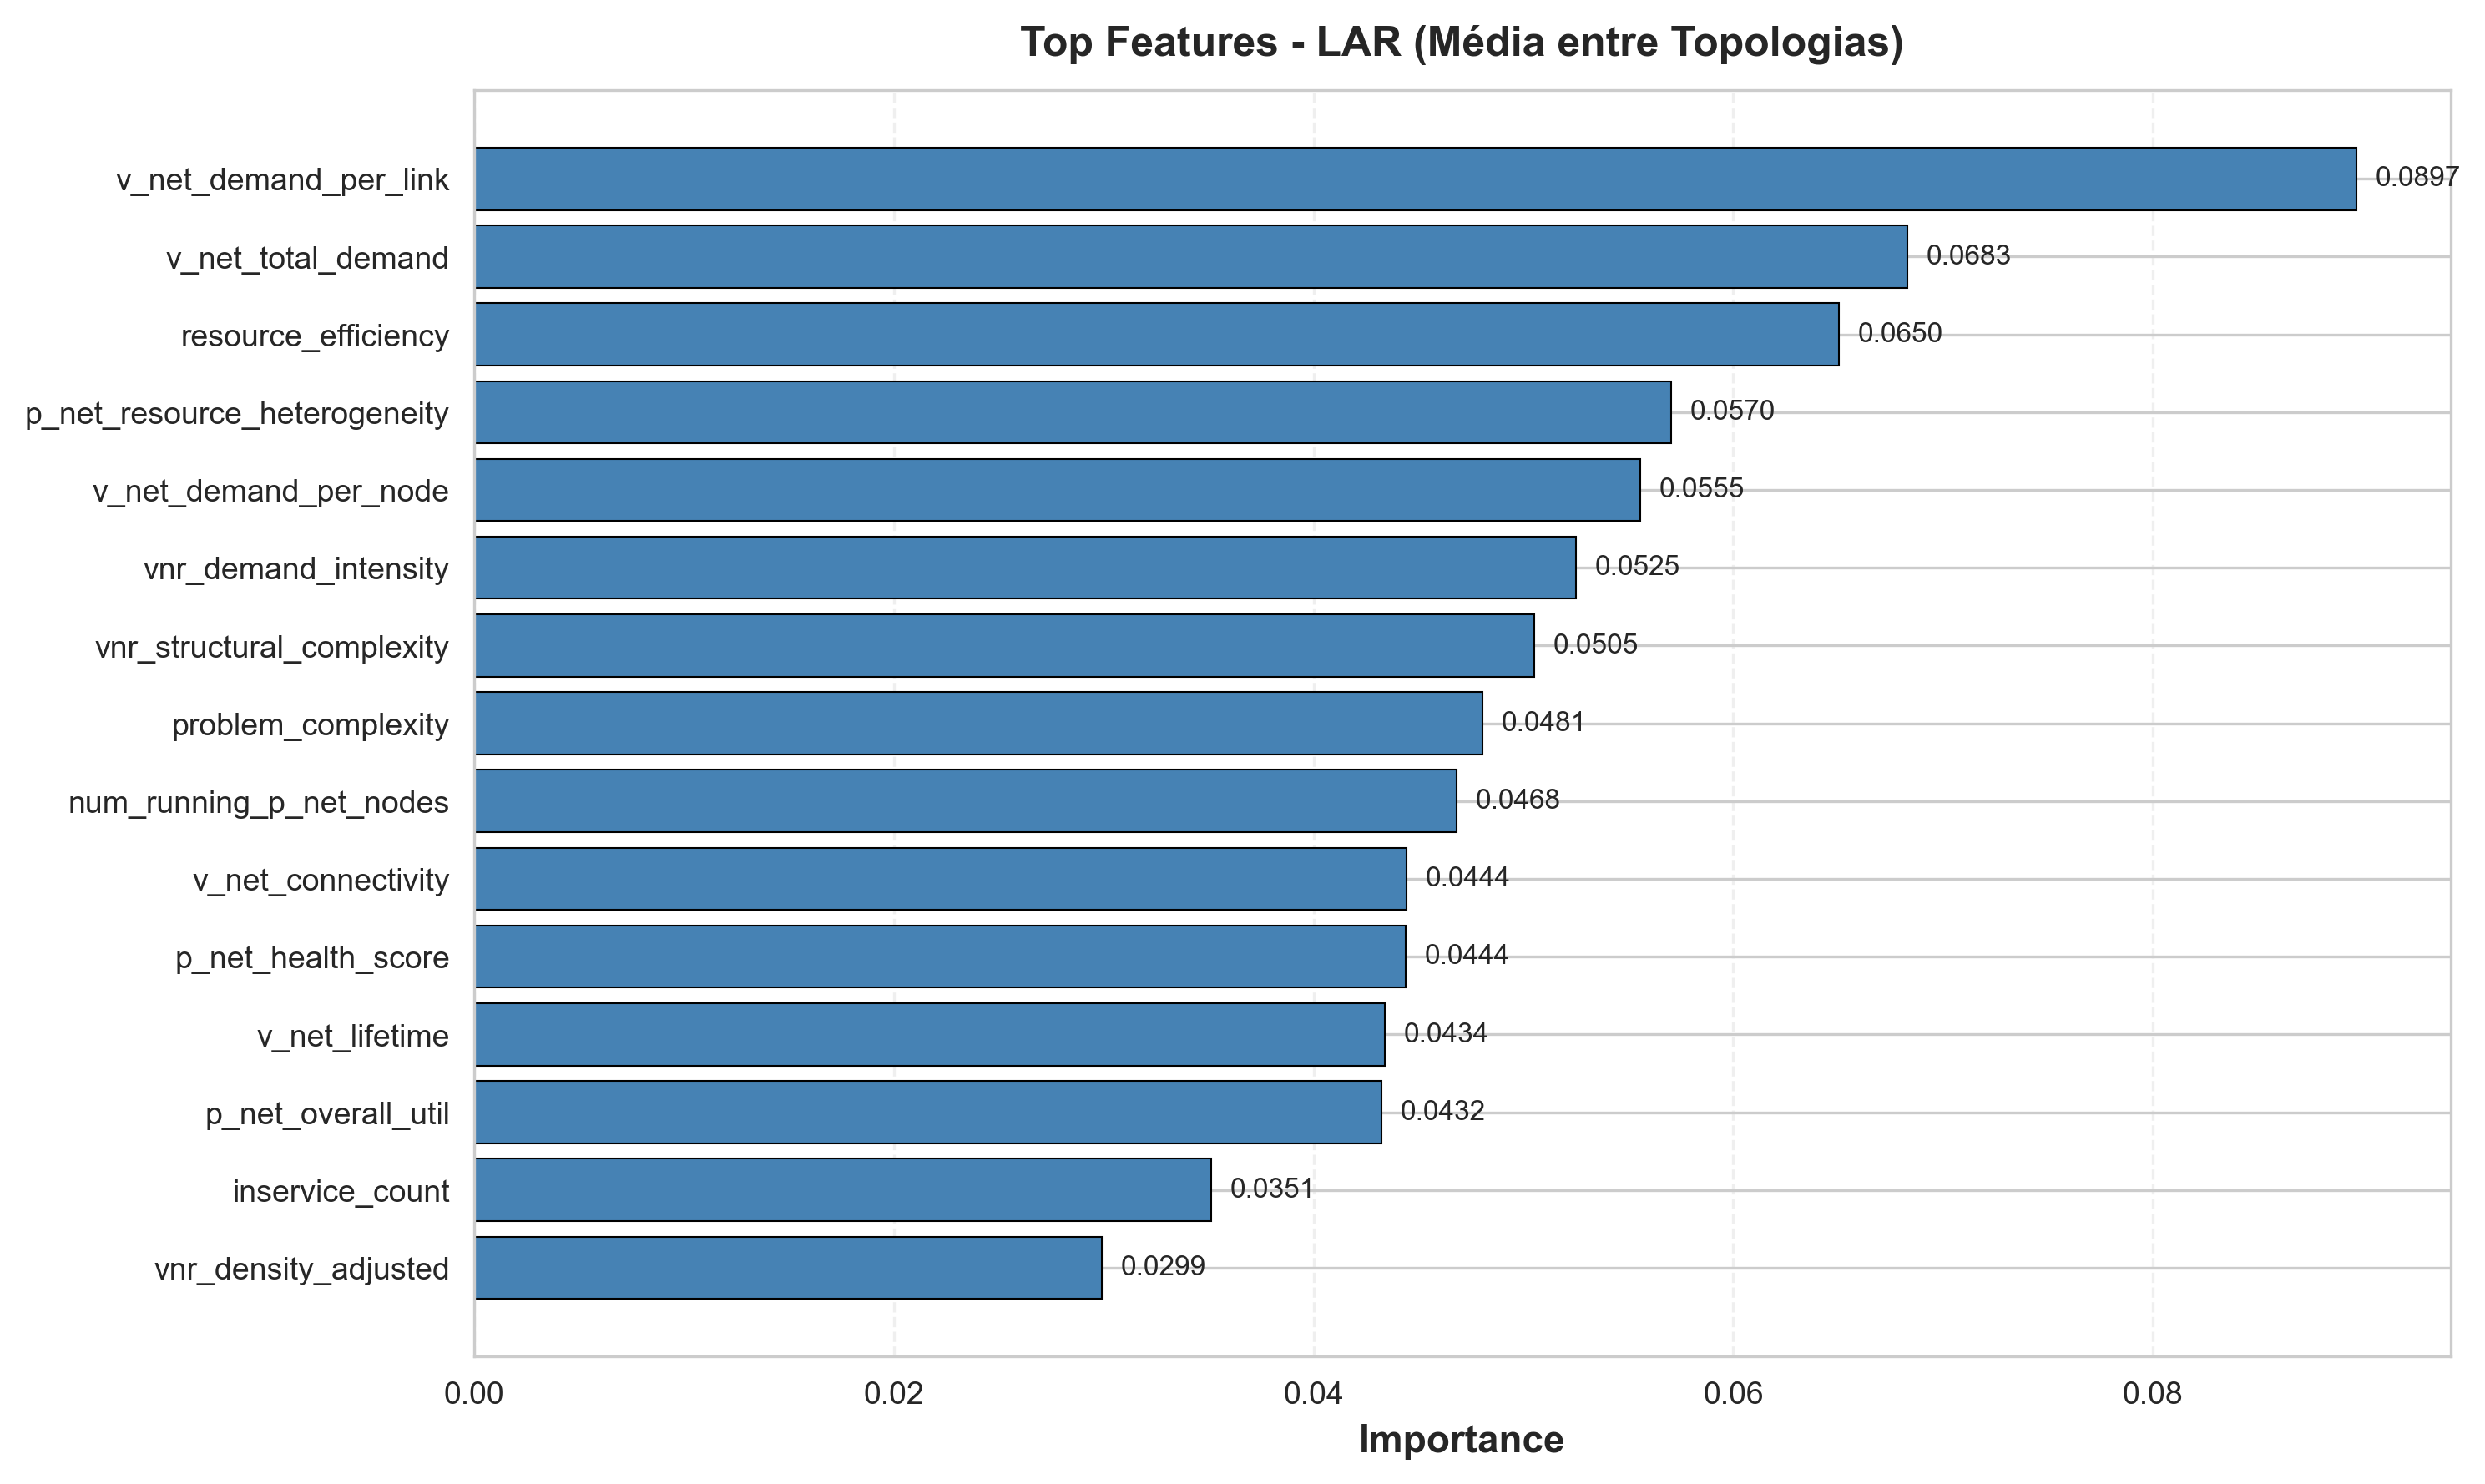
\includegraphics[width=0.95\columnwidth]{per_objective_lar}
    \caption{Importância de Features - LAR (Long-Term Average Revenue). As top 15 features mais importantes (média entre topologias) para o objetivo LAR. A demanda por link da VNR ($v\_net\_demand\_per\_link$) é a feature mais importante com 0,090, seguida pela demanda total ($v\_net\_total\_demand$) com 0,068.}
    \label{fig:feature-importance-lar}
\end{figure}


Esta interpretabilidade é crítica, pois permite que reguladores realizem auditorias ao verificar decisões tomadas pelo sistema, facilita o trabalho de debug ao possibilitar que operadores compreendam o comportamento do sistema, além de aumentar a confiança e a aceitação da automação zero-touch.

\subsection{Latência de Inferência}

Medições de latência de predição para cada modelo (baseadas em benchmark com 10.000 iterações):

\begin{itemize}
    \item \textbf{Tempo médio}: 0,034\,ms por predição
    \item \textbf{Percentil p99}: 0,055\,ms (pior caso: 0,119\,ms)
    \item \textbf{Comparação RL}: FlagVNE requer 50-200\,ms por decisão~\cite{ijcai-2024-flagvne}
\end{itemize}

A Figura~\ref{fig:inference-latency-cdf} apresenta a função de distribuição cumulativa (CDF) da latência de inferência, comparando a abordagem proposta com FlagVNE. Os resultados mostram que mais de 99\% das predições são realizadas em menos de 0,06\,ms, demonstrando consistência na latência sub-milissegundo.

\begin{figure}[H]
\centering
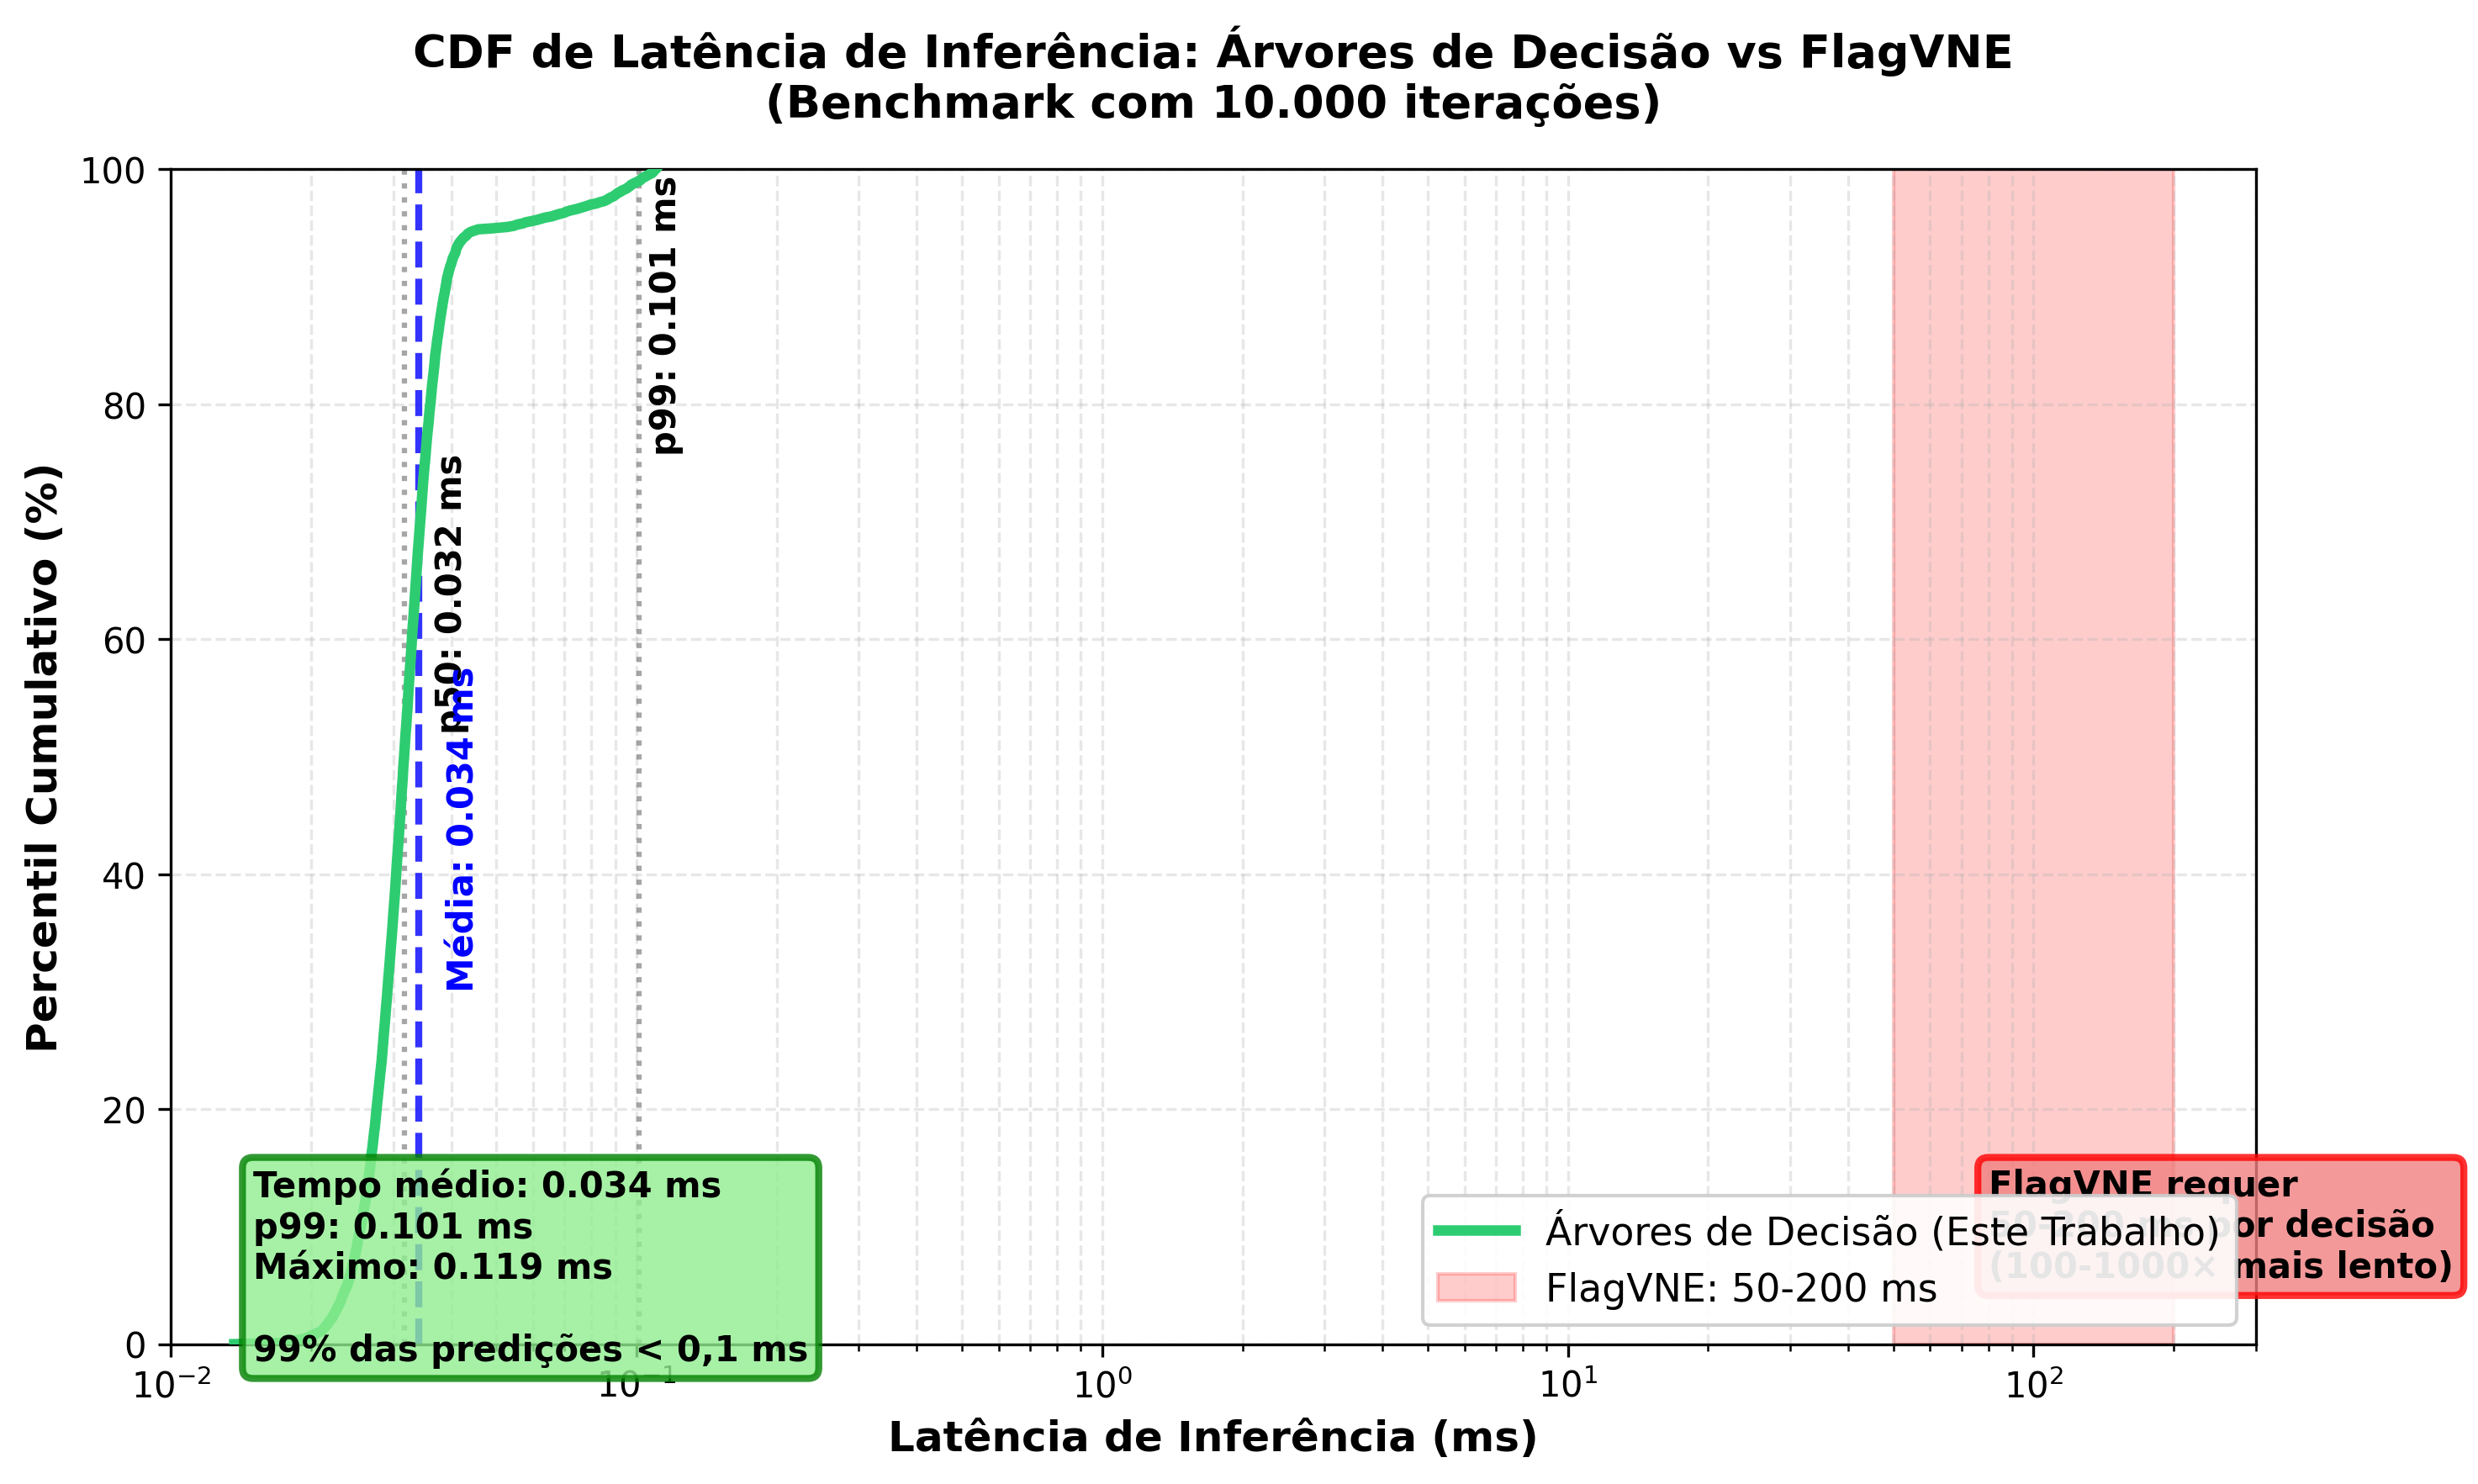
\includegraphics[width=0.95\columnwidth]{inference_latency_cdf}
\caption{CDF de Latência de Inferência: Árvores de Decisão vs FlagVNE. A abordagem proposta apresenta latência consistentemente inferior a 0,1\,ms, enquanto FlagVNE requer 50-200\,ms por decisão (escala diferente no eixo secundário).}
\label{fig:inference-latency-cdf}
\end{figure}

Latência sub-ms viabiliza tomada de decisão online em tempo real, crítica para operação zero-touch.

\section{Conclusão}
\label{sec:Conclusion}

Este trabalho propôs uma abordagem para seleção \textit{zero-touch} de algoritmos de \textit{Virtual Network Embedding} utilizando árvores de decisão multi-objetivo, considerando características das requisições de rede virtual e estado da infraestrutura física.
A abordagem diferencia-se de alternativas baseadas em aprendizado profundo ao oferecer interpretabilidade completa através de caminhos de decisão explícitos e latência de inferência inferior a 1\,ms, viabilizando operação \textit{online} em tempo real.

Especificamente, os resultados experimentais mostram que os fundamentos da abordagem proposta (árvores de decisão, otimização multi-objetivo e interpretabilidade) são candidatos potenciais para alcançar controle de rede \textit{zero-touch} conforme padrão ETSI ZSM.
A análise experimental, baseada em três topologias de \textit{datacenter} (Tree, Fat-Tree e Waxman-16) com 8.000 requisições de rede virtual, mostrou que a seleção contextual de algoritmos pode diminuir tempo de processamento e melhorar taxa de aceitação em vários cenários, sem requerer atualização de software nos pontos finais da infraestrutura.

Os resultados mostram que a abordagem proposta, operando em conjunto com algoritmos tradicionais de VNE como MIP, GA-Meta e PL-Rank, consegue melhorar significativamente o desempenho operacional:
\begin{itemize}
    \item \textbf{Melhoria de Taxa de Aceitação}: Aumento de +89,83\% em relação ao \textit{baseline} de algoritmo fixo (de 43,17\% para 81,95\%)
    \item \textbf{Top-3 Accuracy}: Entre 79,1\% e 85,9\%, mostrando robustez na predição do melhor algoritmo
    \item \textbf{Melhoria de Razão Receita-Custo}: Aumento de +58,76\% (de 0,4574 para 0,7262)
    \item \textbf{Melhoria de Receita Média}: Aumento de +61,40\% (de 70,29 para 113,45 por VNR)
\end{itemize}

As técnicas de balanceamento de classes empregadas (pesos customizados $1/\sqrt{f}$ e ajuste de hiperparâmetros) foram essenciais para capturar padrões de classes minoritárias, resultando em F1-Macro de 0,56 para o objetivo RAC.
Além disso, os resultados experimentais confirmaram empiricamente que nenhum algoritmo VNE é universalmente ótimo, validando a necessidade de seleção contextual baseada em características das requisições e estado da rede.

Como limitações, o modelo foi treinado em três topologias simuladas e as características capturam estado instantâneo da rede.
Como trabalhos futuros, direções promissoras incluem \textit{transfer learning} entre topologias, incorporação de histórico temporal de requisições, e validação em ambientes de produção com cargas de trabalho reais de \textit{datacenter}.

%===================================================================

\bibliographystyle{IEEEtran}
\bibliography{references}

\end{document}